\section{Messergebnisse und Auswertung}

\subsection{Vorgehensweise bei der Auswertung}
\autoref{img:ex:both} zeigt beispielhaft das Signal einer Messung mit dem SQUID. Man erkennt, dass das Messignal in zwei, vertikal verschobene 
Sinuskurven aufgespalten ist. Da dies für einen sinnvollen Fit ungünstig ist, wird für alle Messignale nur das obere Signal gefittet. 
Wir gehen davon aus, dass der Fit des unteren Signals oder die Bildung des Mittelwerts der beiden Signale das gleiche Ergebnis liefert.
\begin{figure}[H]
\begin{center}
  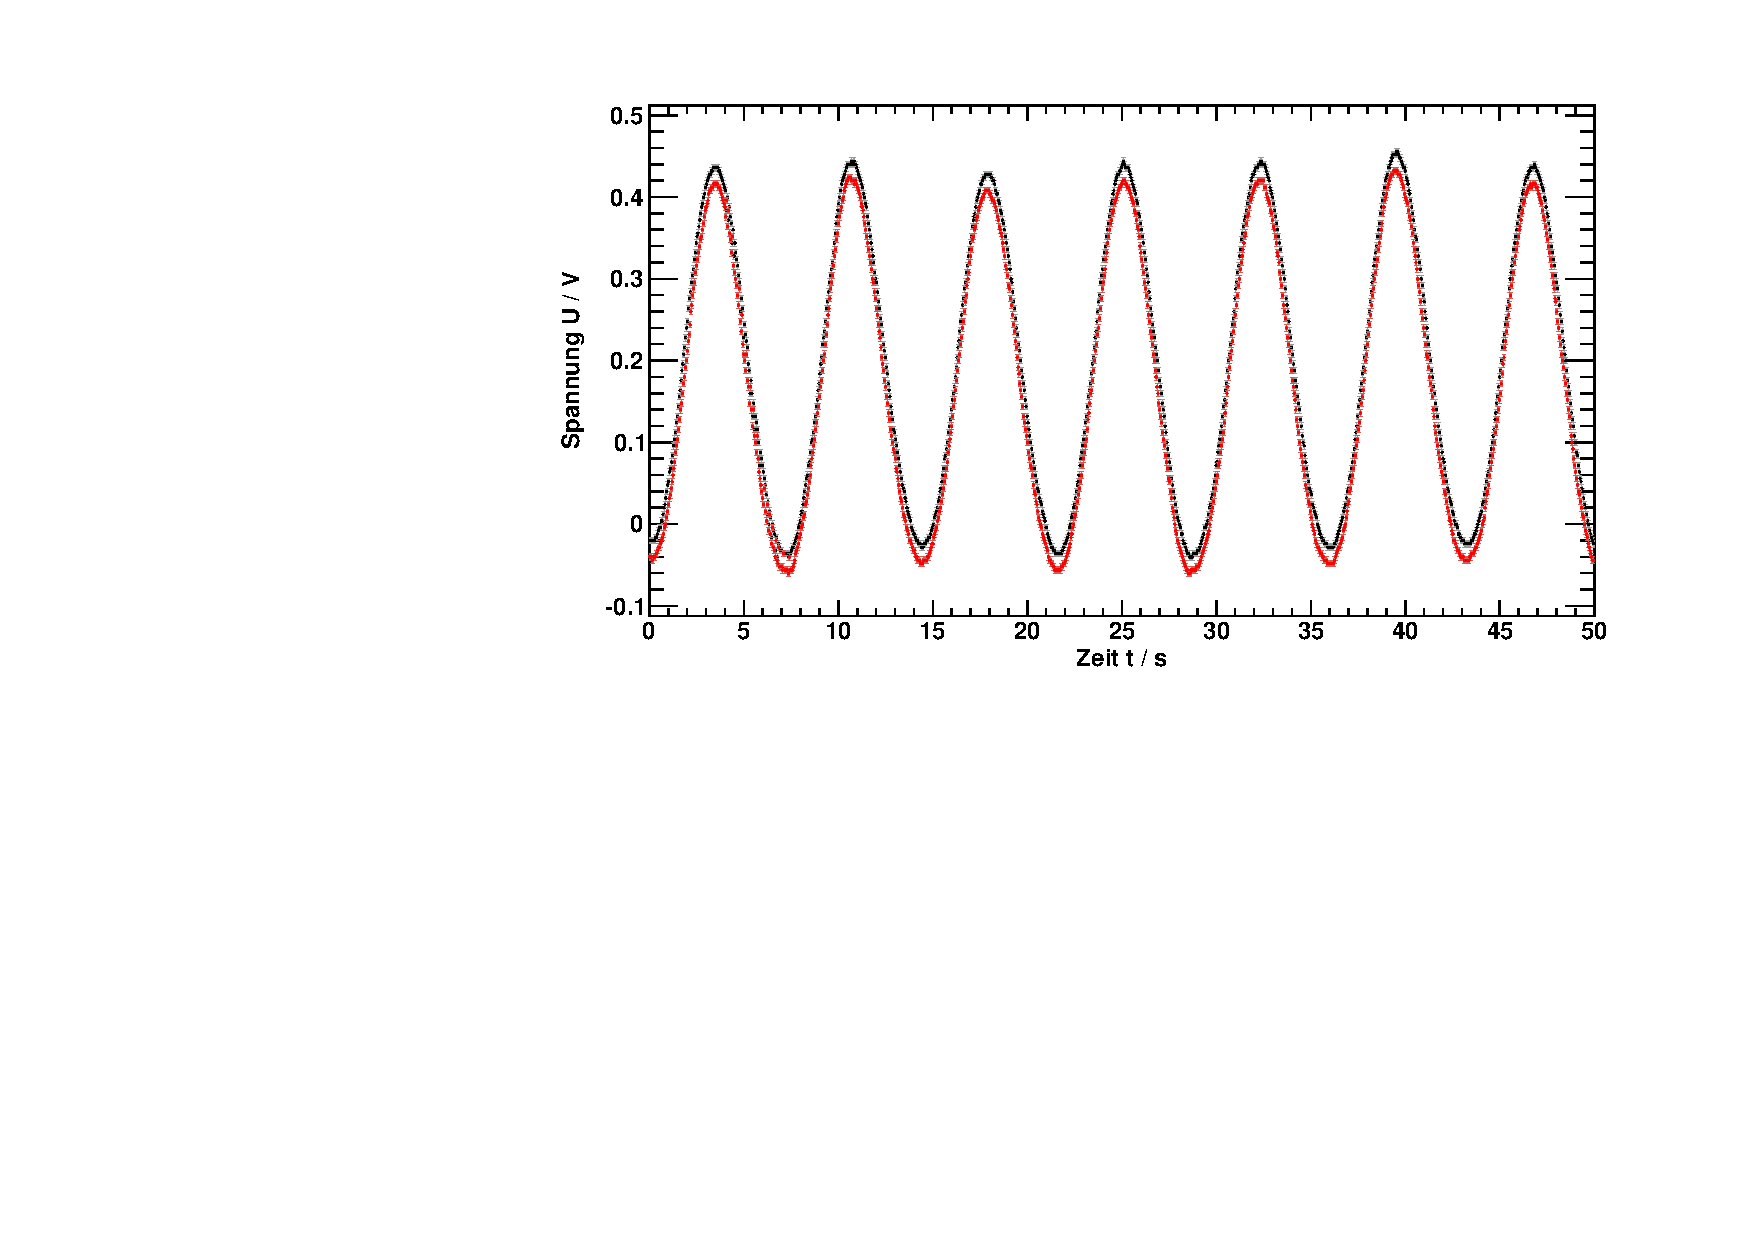
\includegraphics[width=0.9\textwidth]{../img/both_Spule_R1.pdf}
  \caption{\emph{SQUID}-Signal der stromdurchflossenen Leiterschleife mit R1 als Widerstand.
  Der Grund für die Aufspaltung in zwei vertikal verschobene Sinuskurven ist nicht bekannt.}
  \label{img:ex:both}
\end{center}
\end{figure}

Das obere Signal wird mit einer allgemeinen Sinuskurve
\begin{equation}
  \label{eq:fit}
  U(t) = A \cdot \sin(\omega \cdot t + \phi) + c
\end{equation}
gefittet. Dabei ist $A$ die Amplitude, $\omega$ die Kreisfrequenz, $\phi$ ein konstanter Phasenoffset und $c$ ein konstanter Spannungsoffset.
Dieser Ansatz ist sinnvoll, da die Probe rotiert wird und somit auch ein periodisches Signal erwartet werden kann. \\
Ein Beispiel für einen Fit ist in \autoref{img:ex:fit} dargestellt. Der $\chi^2$-Wert ist überhöht, weil dem Signal ein Untergrundsignal überlagert 
ist und das sinusförmige Signal somit deformiert wird. \\
Aus der Amplitude $A$ lässt sich nun mit \autoref{eq:AtoB} das maximale Stärke des Magnetfeldes berechnen. Diese Ergebnis wird hier für das 
Beispiel nicht extra angegeben, da die Diskussion der Magnetfeldstärke der Leiterschleife weiter unten erfolgt.

\begin{figure}[H]
\begin{center}
  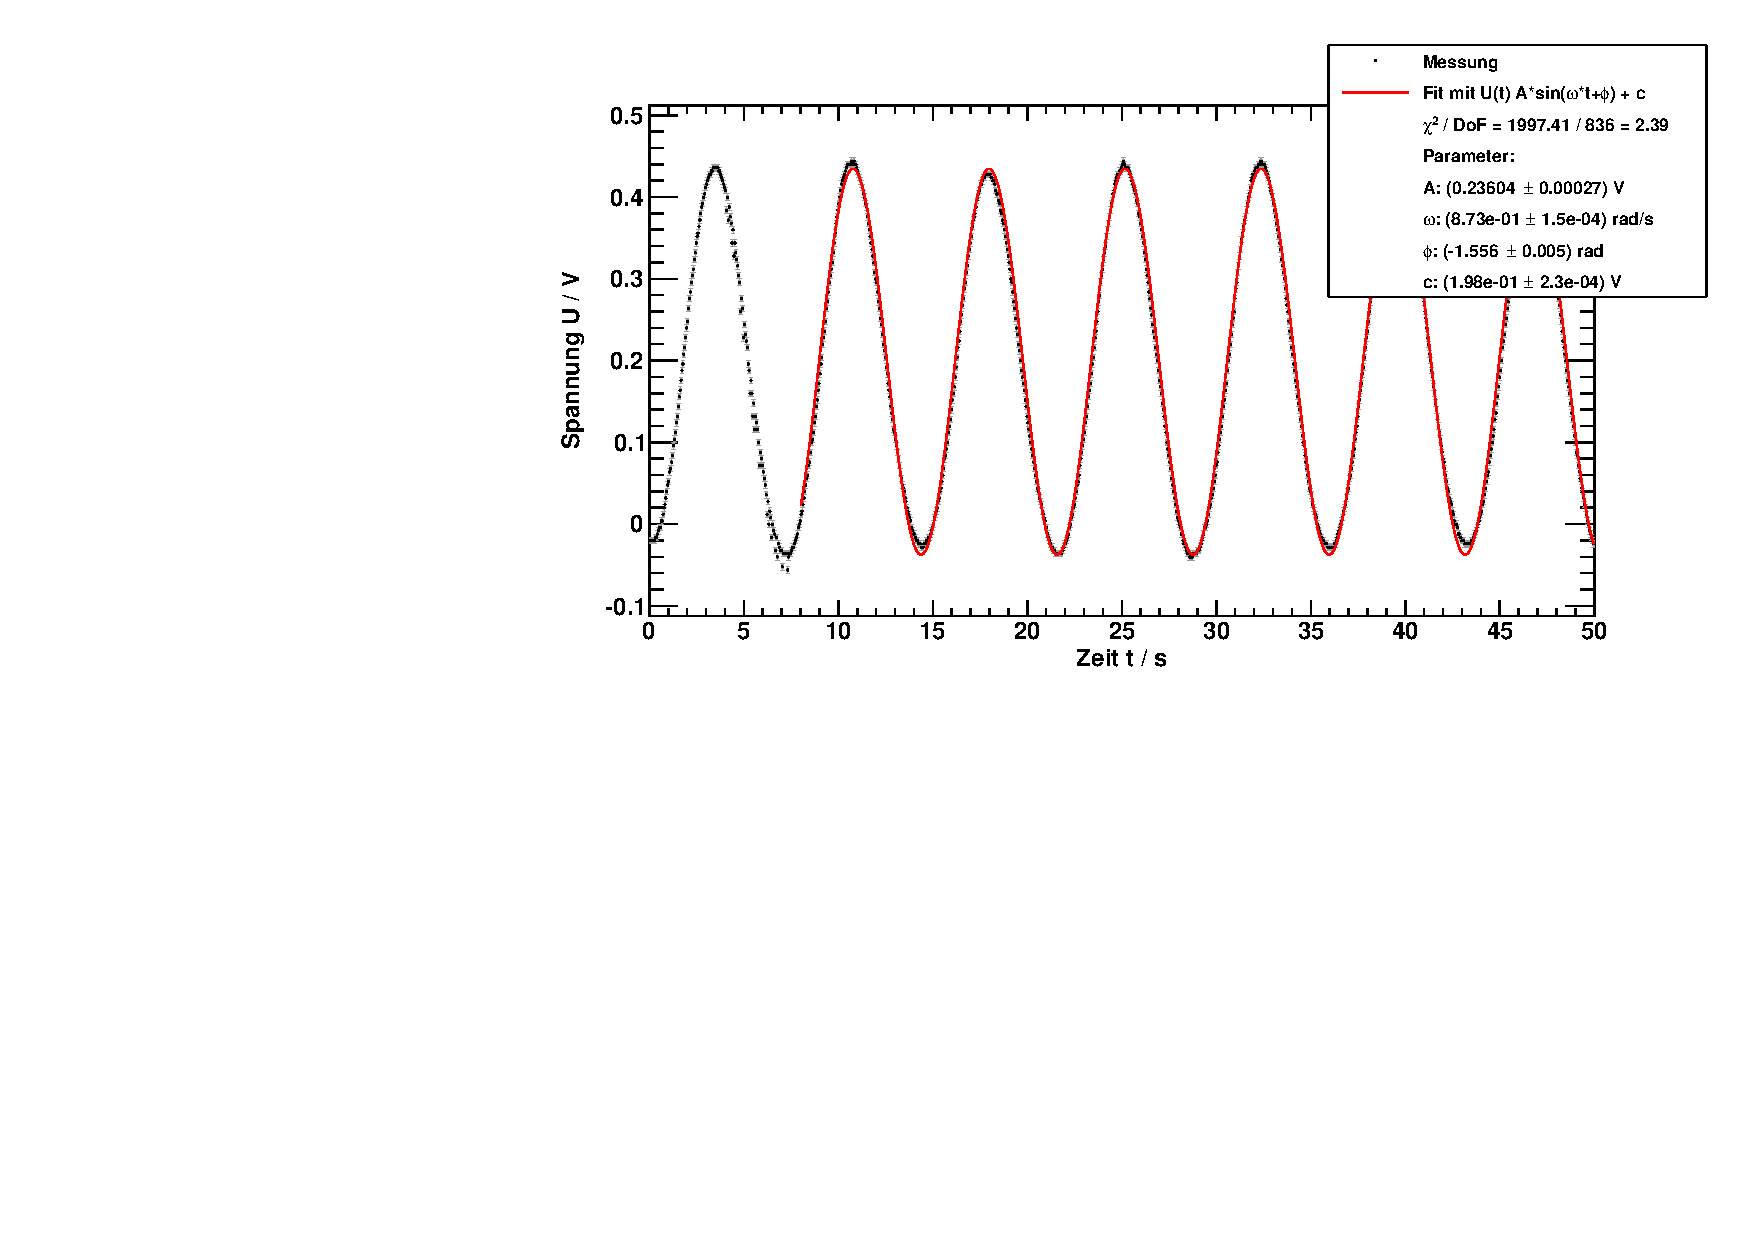
\includegraphics[width=0.9\textwidth]{../img/fit_Spule_R1.pdf}
  \caption{Fit des oberen Signals der Leiterschleife mit R1 als Widerstand mit einer Sinusfunktion.}
  \label{img:ex:fit}
\end{center}
\end{figure}

Mit der Kreisfrequenz $\omega$ und dem Phasenoffset $\phi$ kann nun ein Polarplot des Messsignals durch folgende Transformation erstellt werden.
\begin{equation}
  \label{eq:polartransform}
  \begin{split}
    x(t) &= |B_z(t)| \cdot \cos(\omega \cdot t + \phi) \\
    y(t) &= |B_z(t)| \cdot \sin(\omega \cdot t + \phi)
  \end{split}
\end{equation}
$B_z(t)$ berechnet sich für jeden Zeitpunkt $t$ mit \autoref{eq:AtoB} aus $U'(t)$. Von der eigentlichen Spannung $U'(t)$ muss noch der 
konstante Offset $c$ abgezogen werden, damit die Amplitude um 0 herum oszilliert.
\begin{equation}
  U'(t) = U(t) - c
\end{equation}
Die so erhaltenen Polardarstellung für den Beispielfit sieht man in \autoref{img:ex:polar}
\begin{figure}[H]
\begin{center}
  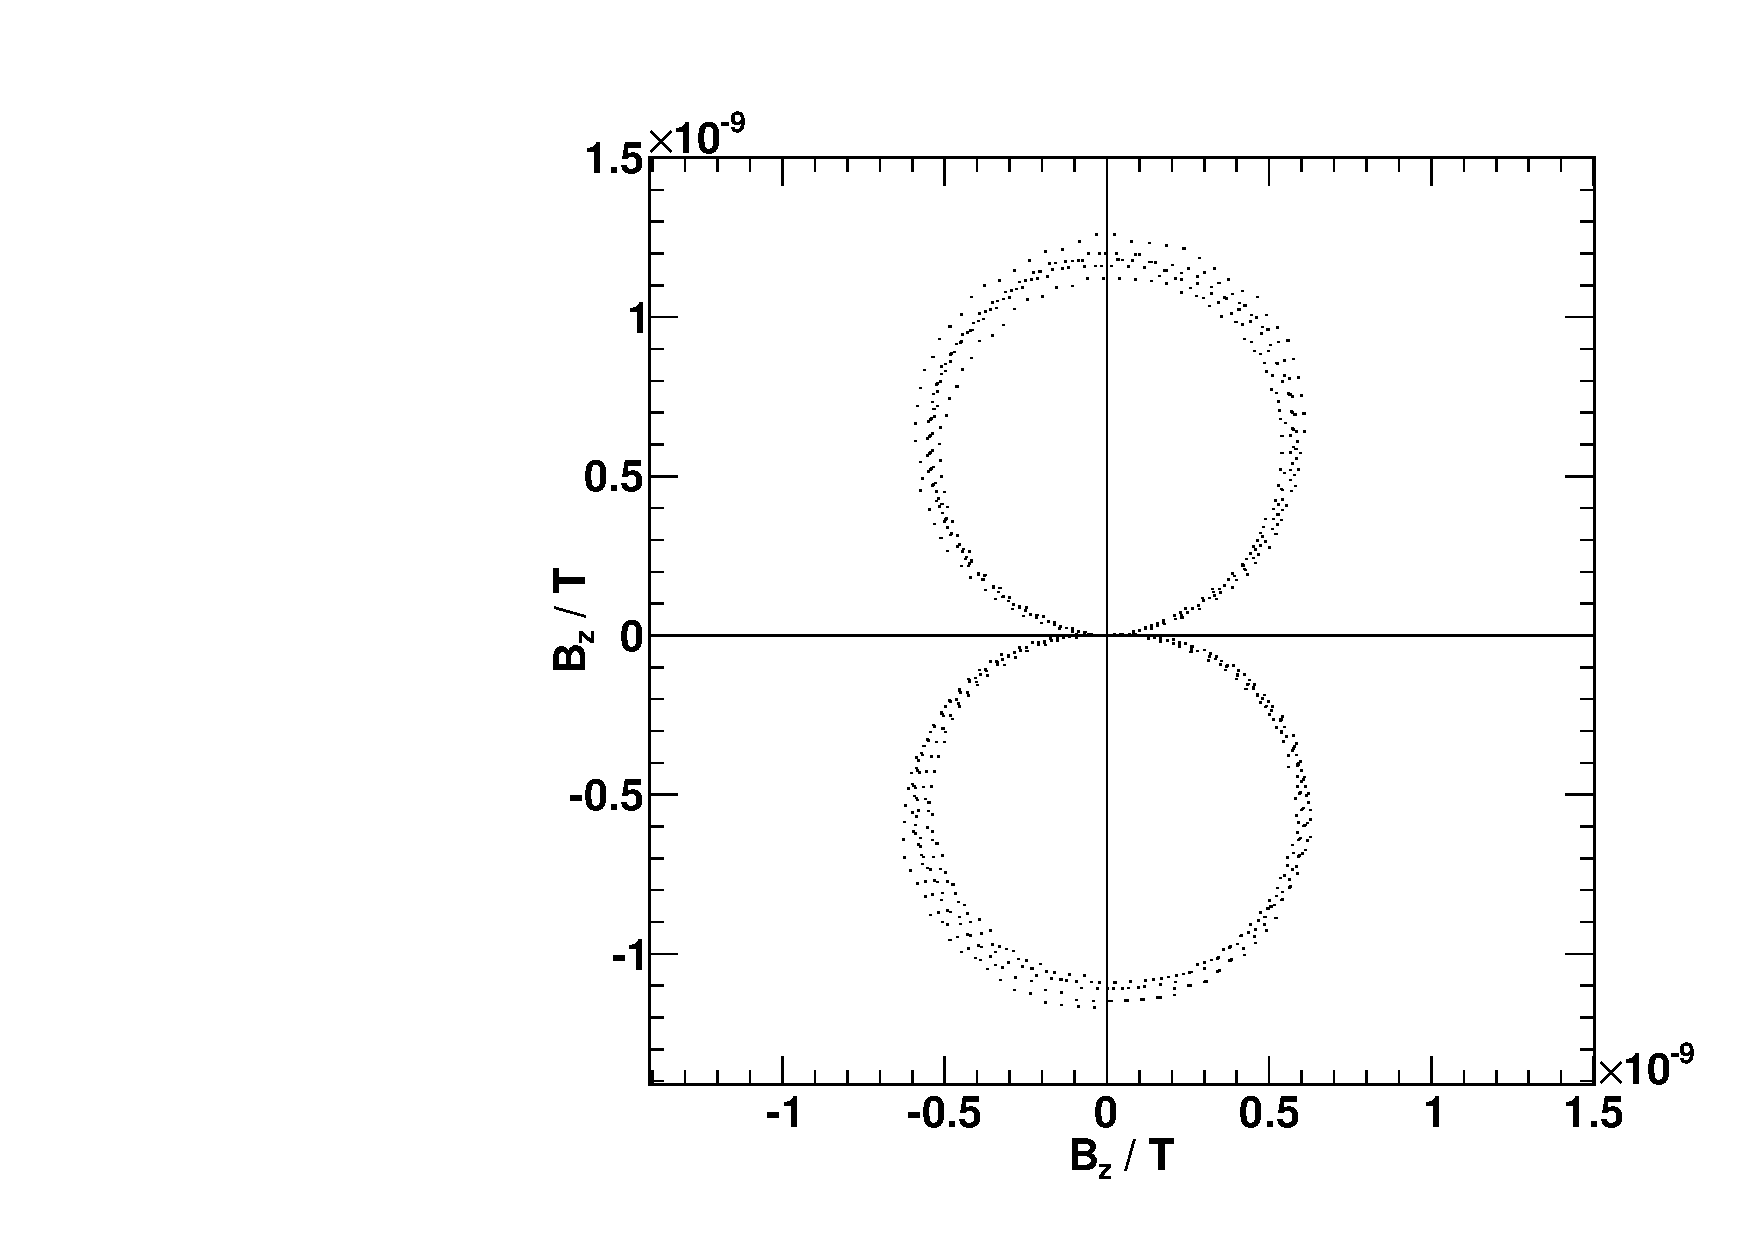
\includegraphics[width=0.6\textwidth]{../img/polar_Spule_R1.pdf}
  \caption{Polarplot der Messdaten aus \autoref{img:ex:fit} mit der Kreisfrequenz $\omega$,
  die aus dem Fit gewonnen wurde: Dipolfeld einer stromdurchflossenen Leiterschleife mit R1 als Widerstand.}
  \label{img:ex:polar}
\end{center}
\end{figure}

\subsection{Vermessung des Magnetfeldes der Leiterschleife}
\subsubsection{Berechnung aus der SQUID-Messung}

Die SQUID-Signale wurden wie oben beschrieben mit einem Sinus gefittet und in einem Polarplot dargestellt 
(\autoref{img:R1} bis \autoref{img:R5}). Bei den Fits wurde jeweils ein Bereich auf der x-Achse gewählt, in dem Amplitude keine zu großen 
Schwankungen aufwies.

\begin{figure}[H]
\begin{center}
  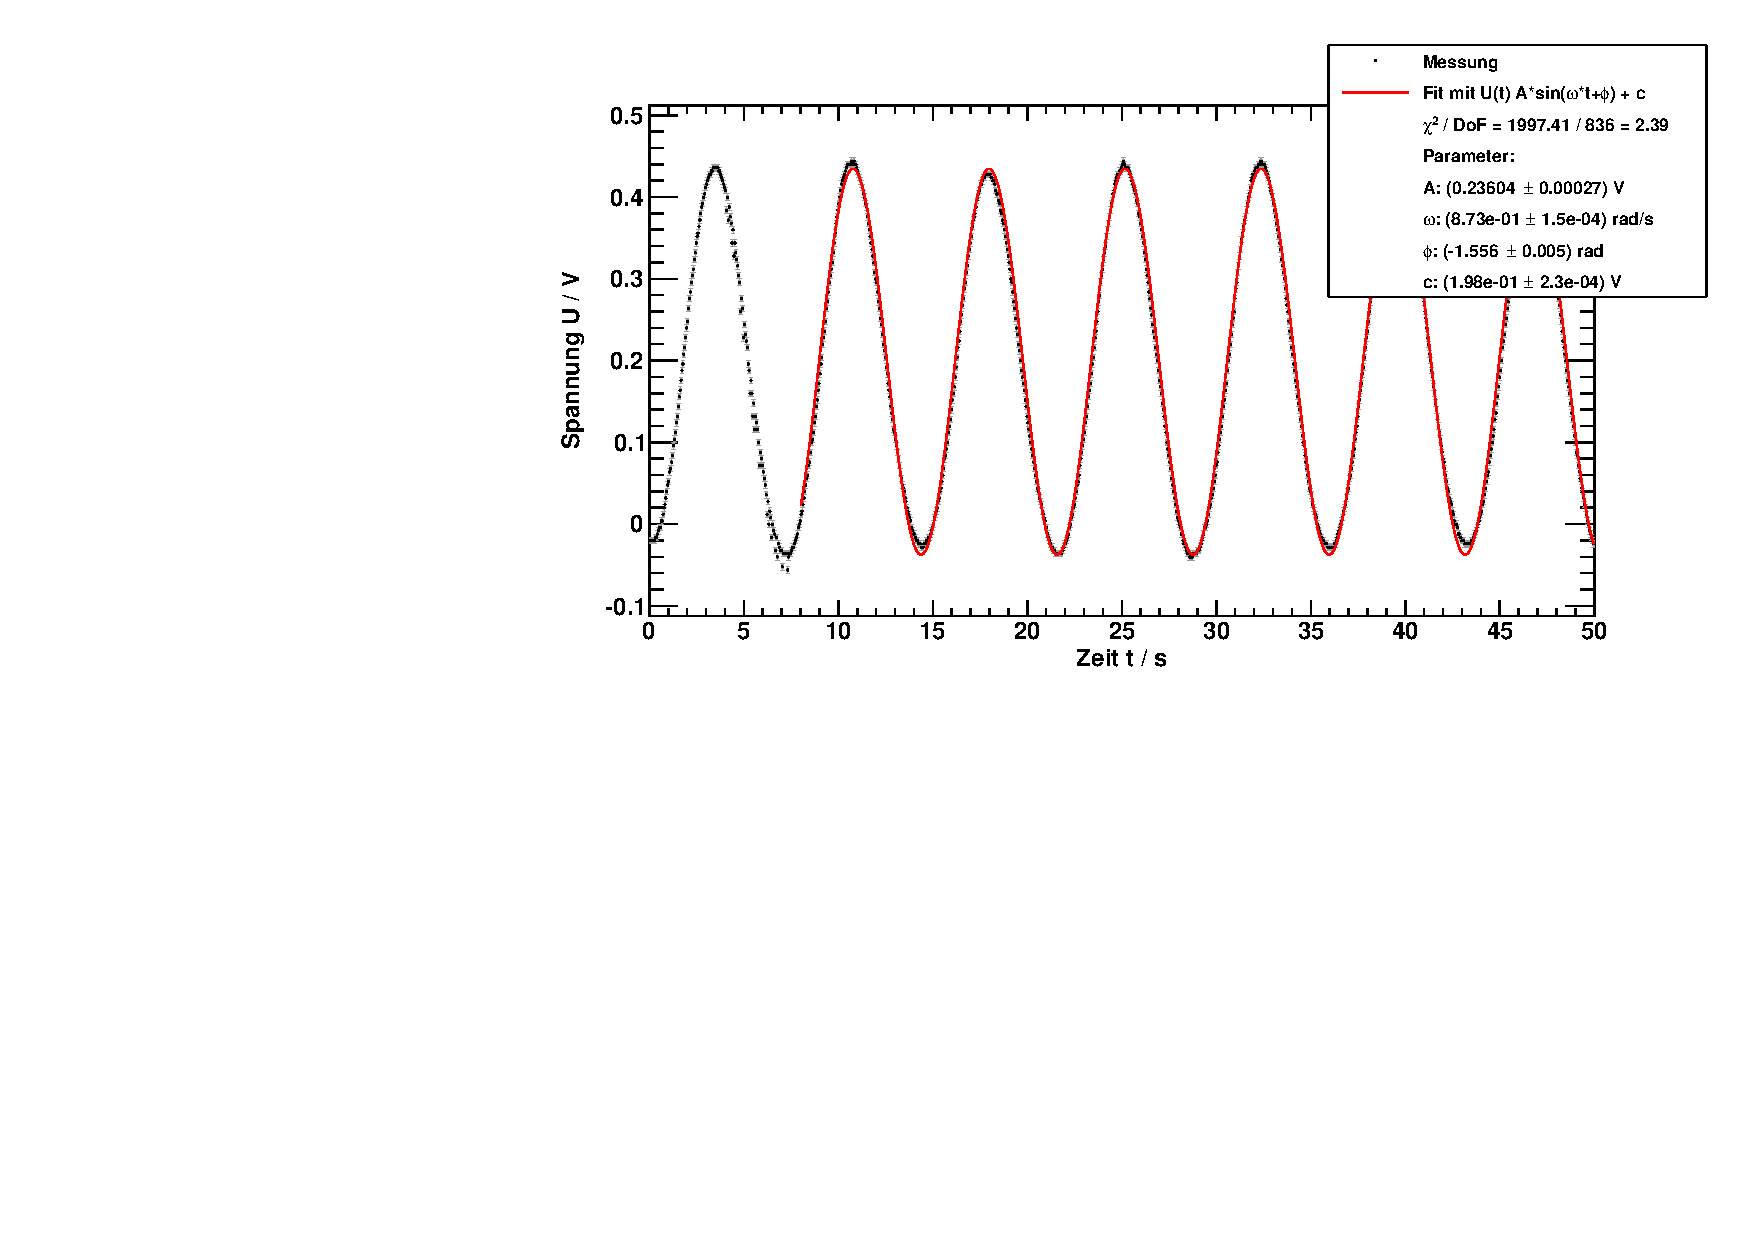
\includegraphics[width=0.64\textwidth]{../img/fit_Spule_R1.pdf}
  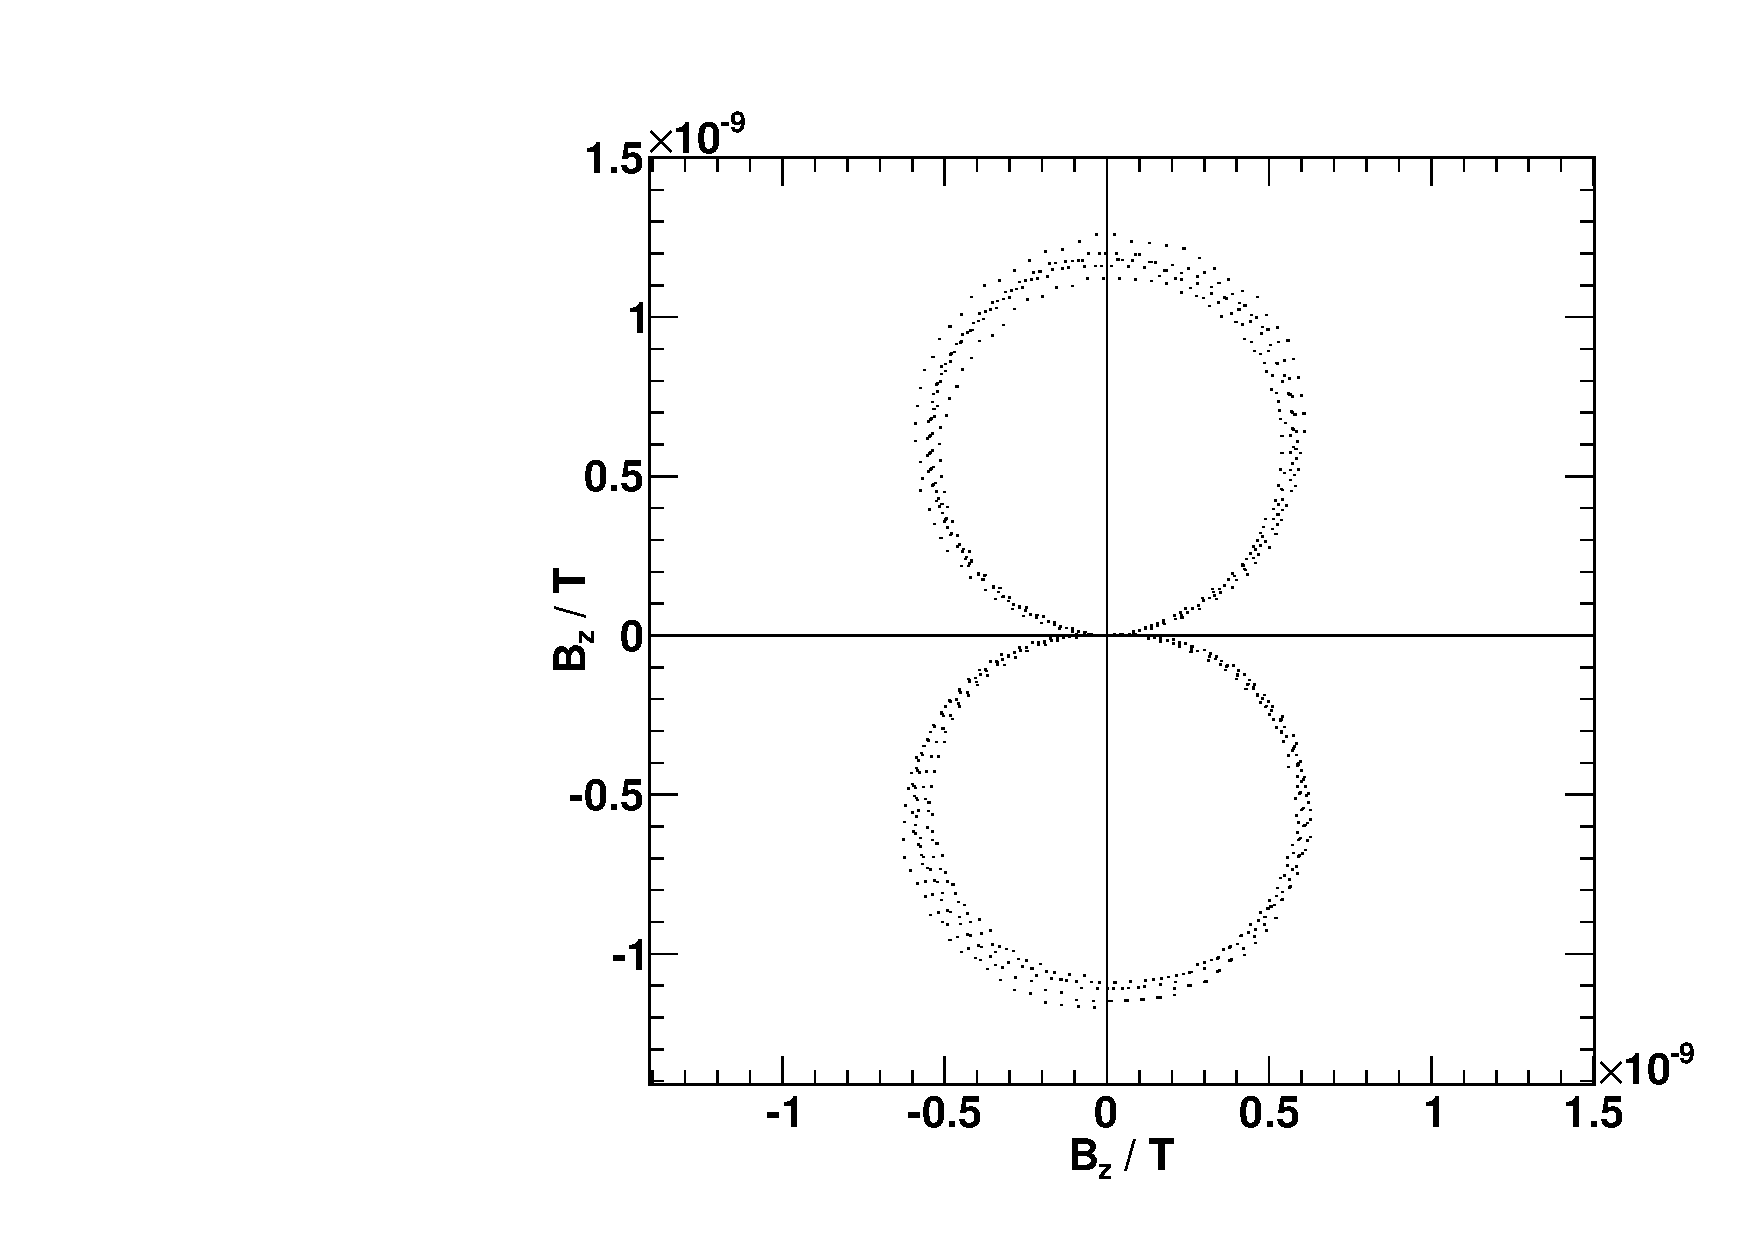
\includegraphics[width=0.35\textwidth]{../img/polar_Spule_R1.pdf}
  \caption{Fit und Polarplot des Magnetfeldes der Leiterschleife mit Widerstand R1.}
  \label{img:R1}
\end{center}
\end{figure}

\begin{figure}[H]
\begin{center}
  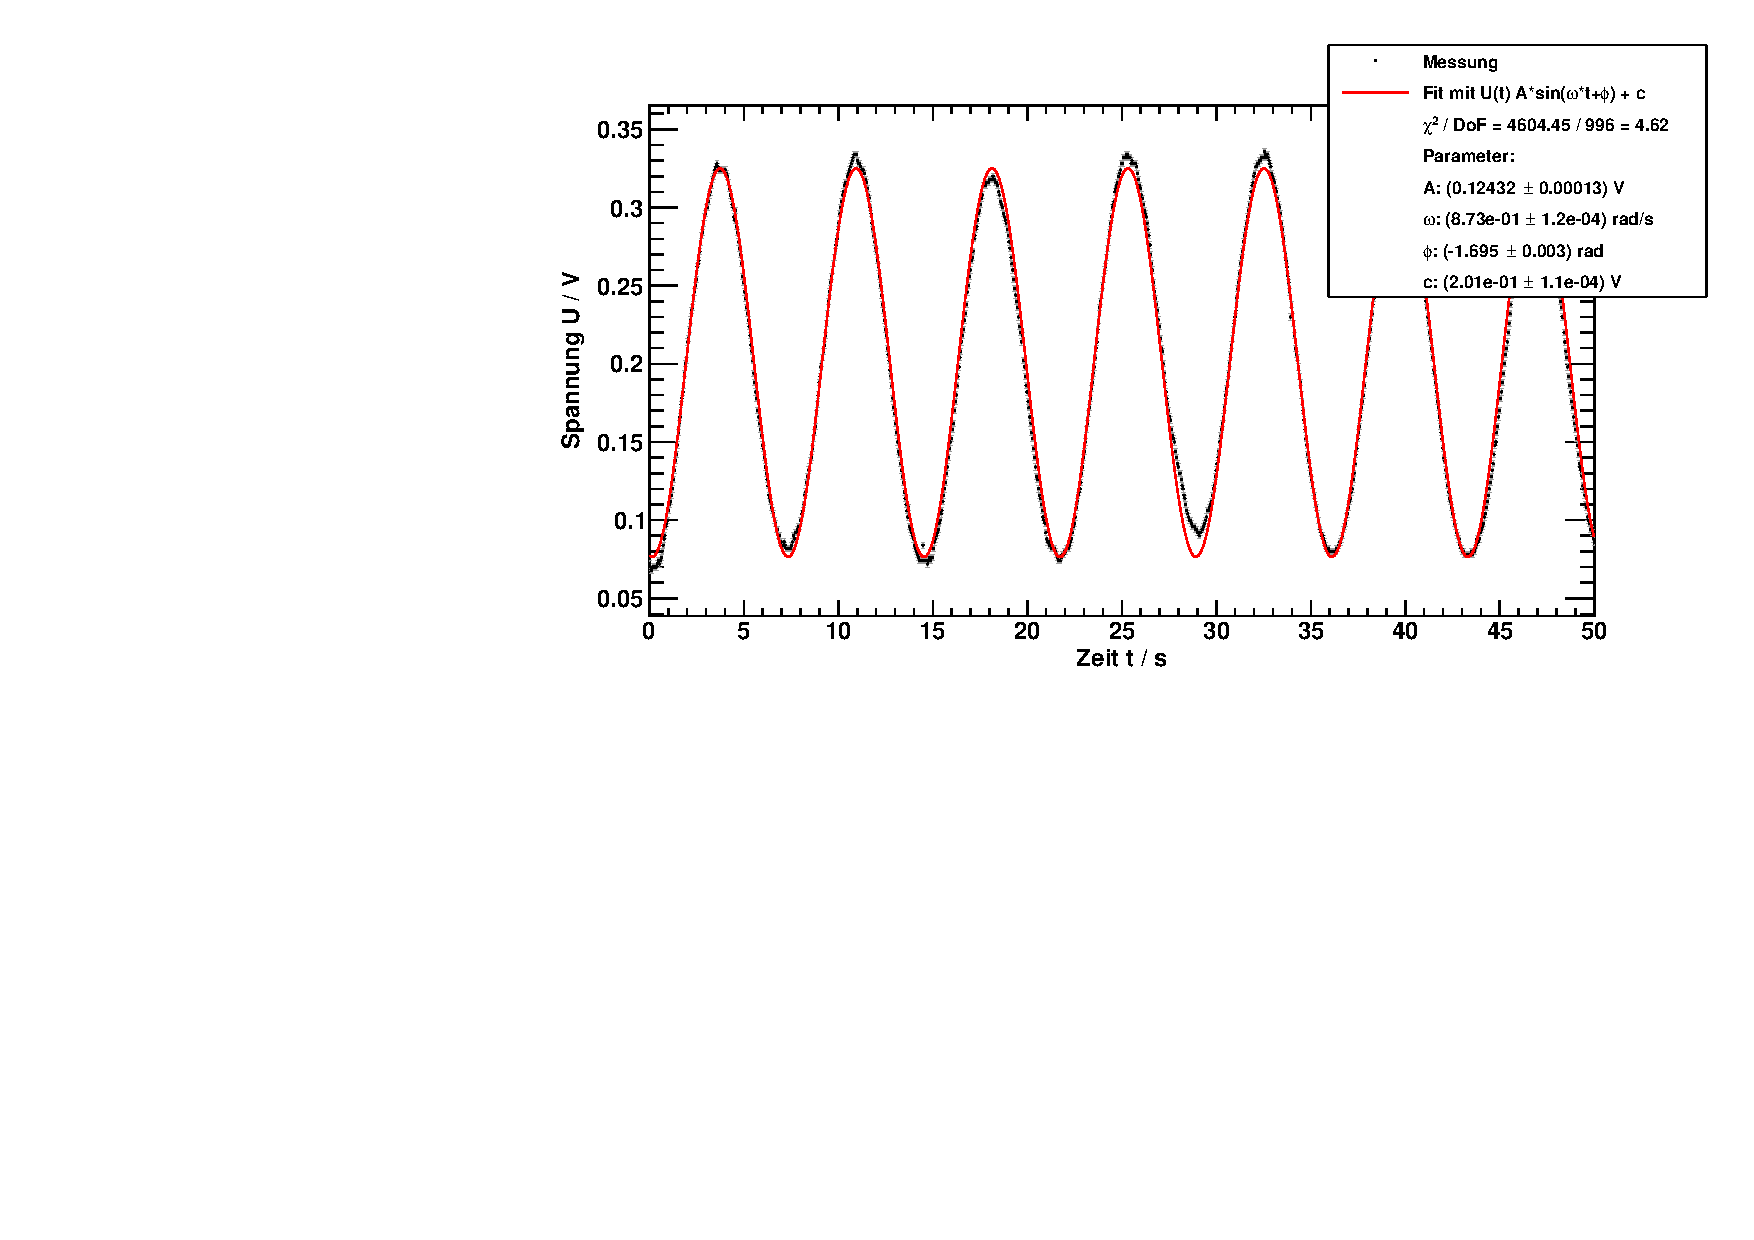
\includegraphics[width=0.64\textwidth]{../img/fit_Spule_R2.pdf}
  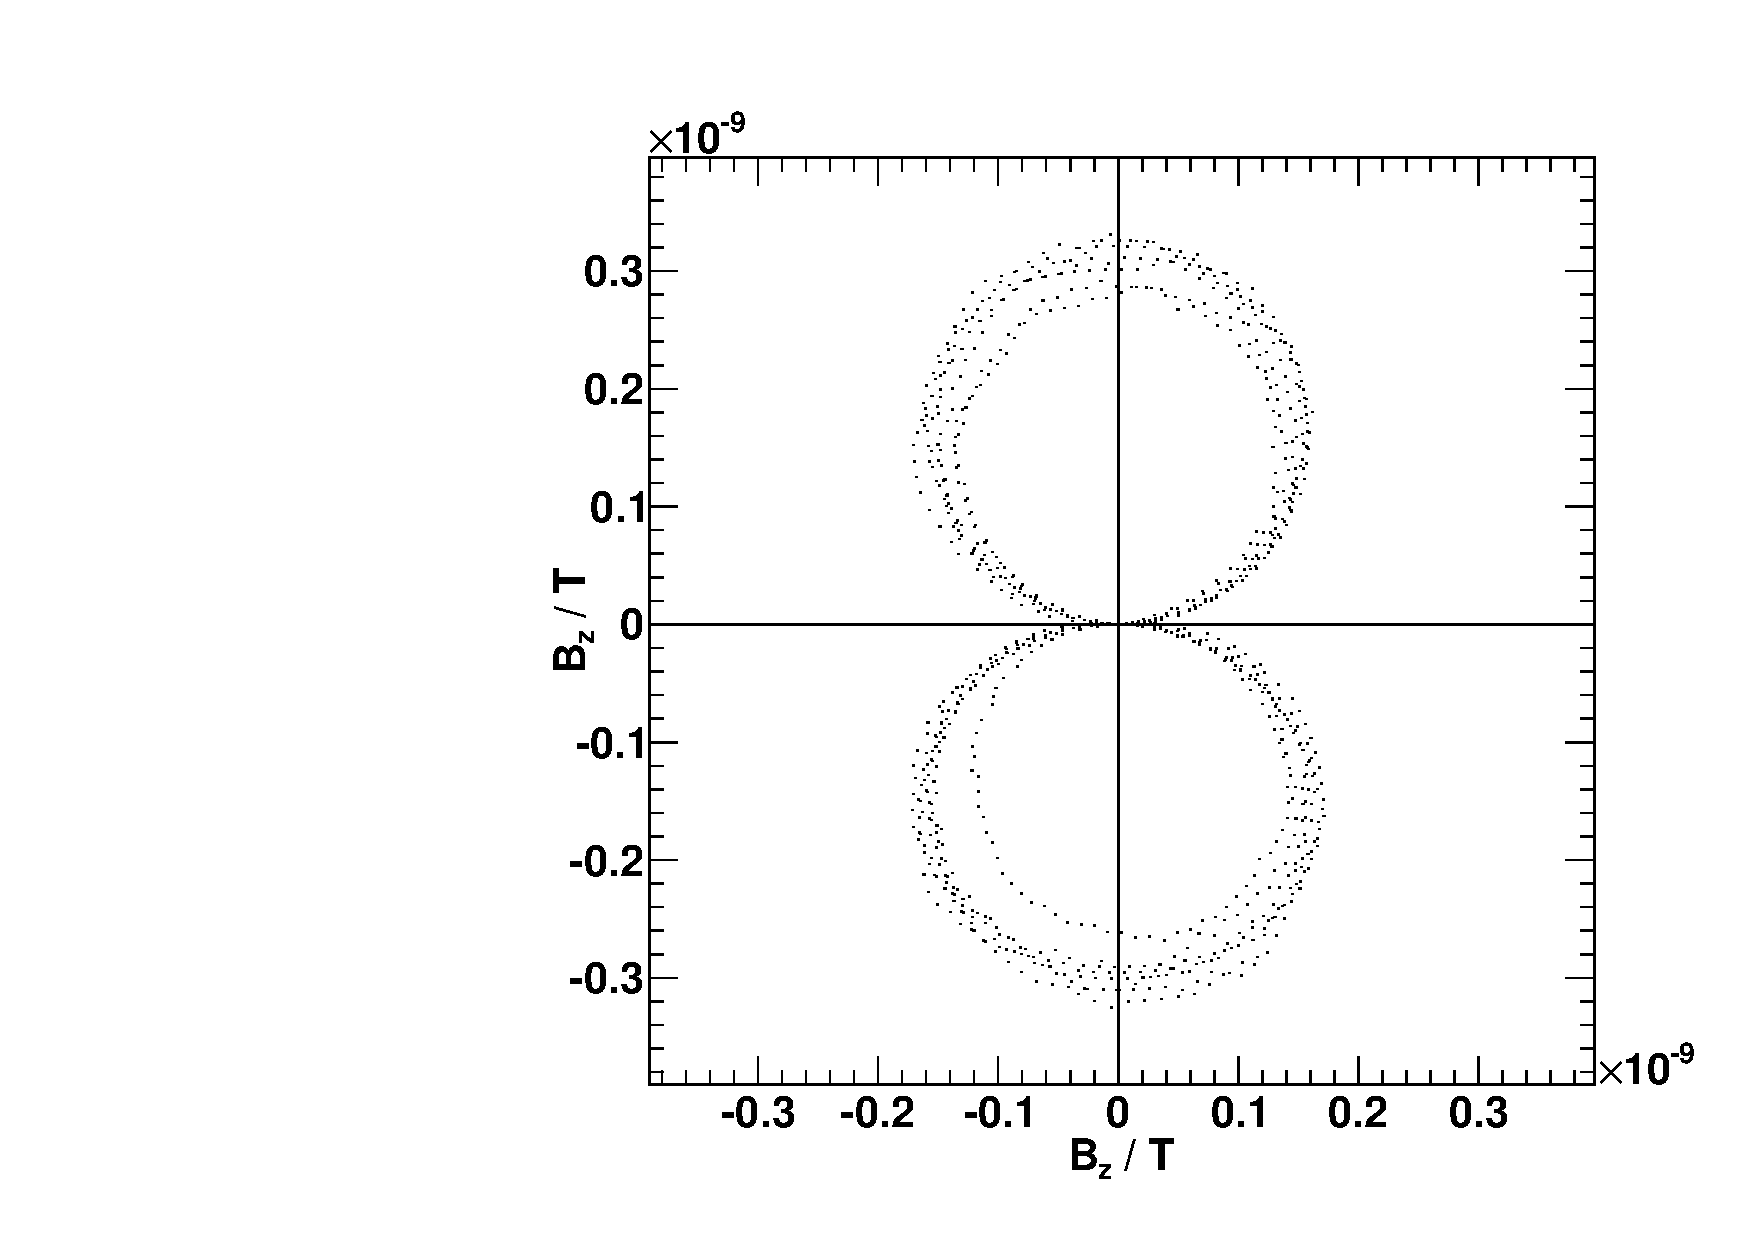
\includegraphics[width=0.35\textwidth]{../img/polar_Spule_R2.pdf}
  \caption{Fit und Polarplot des Magnetfeldes der Leiterschleife mit Widerstand R2.}
  \label{img:R2}
\end{center}
\end{figure}

\begin{figure}[H]
\begin{center}
  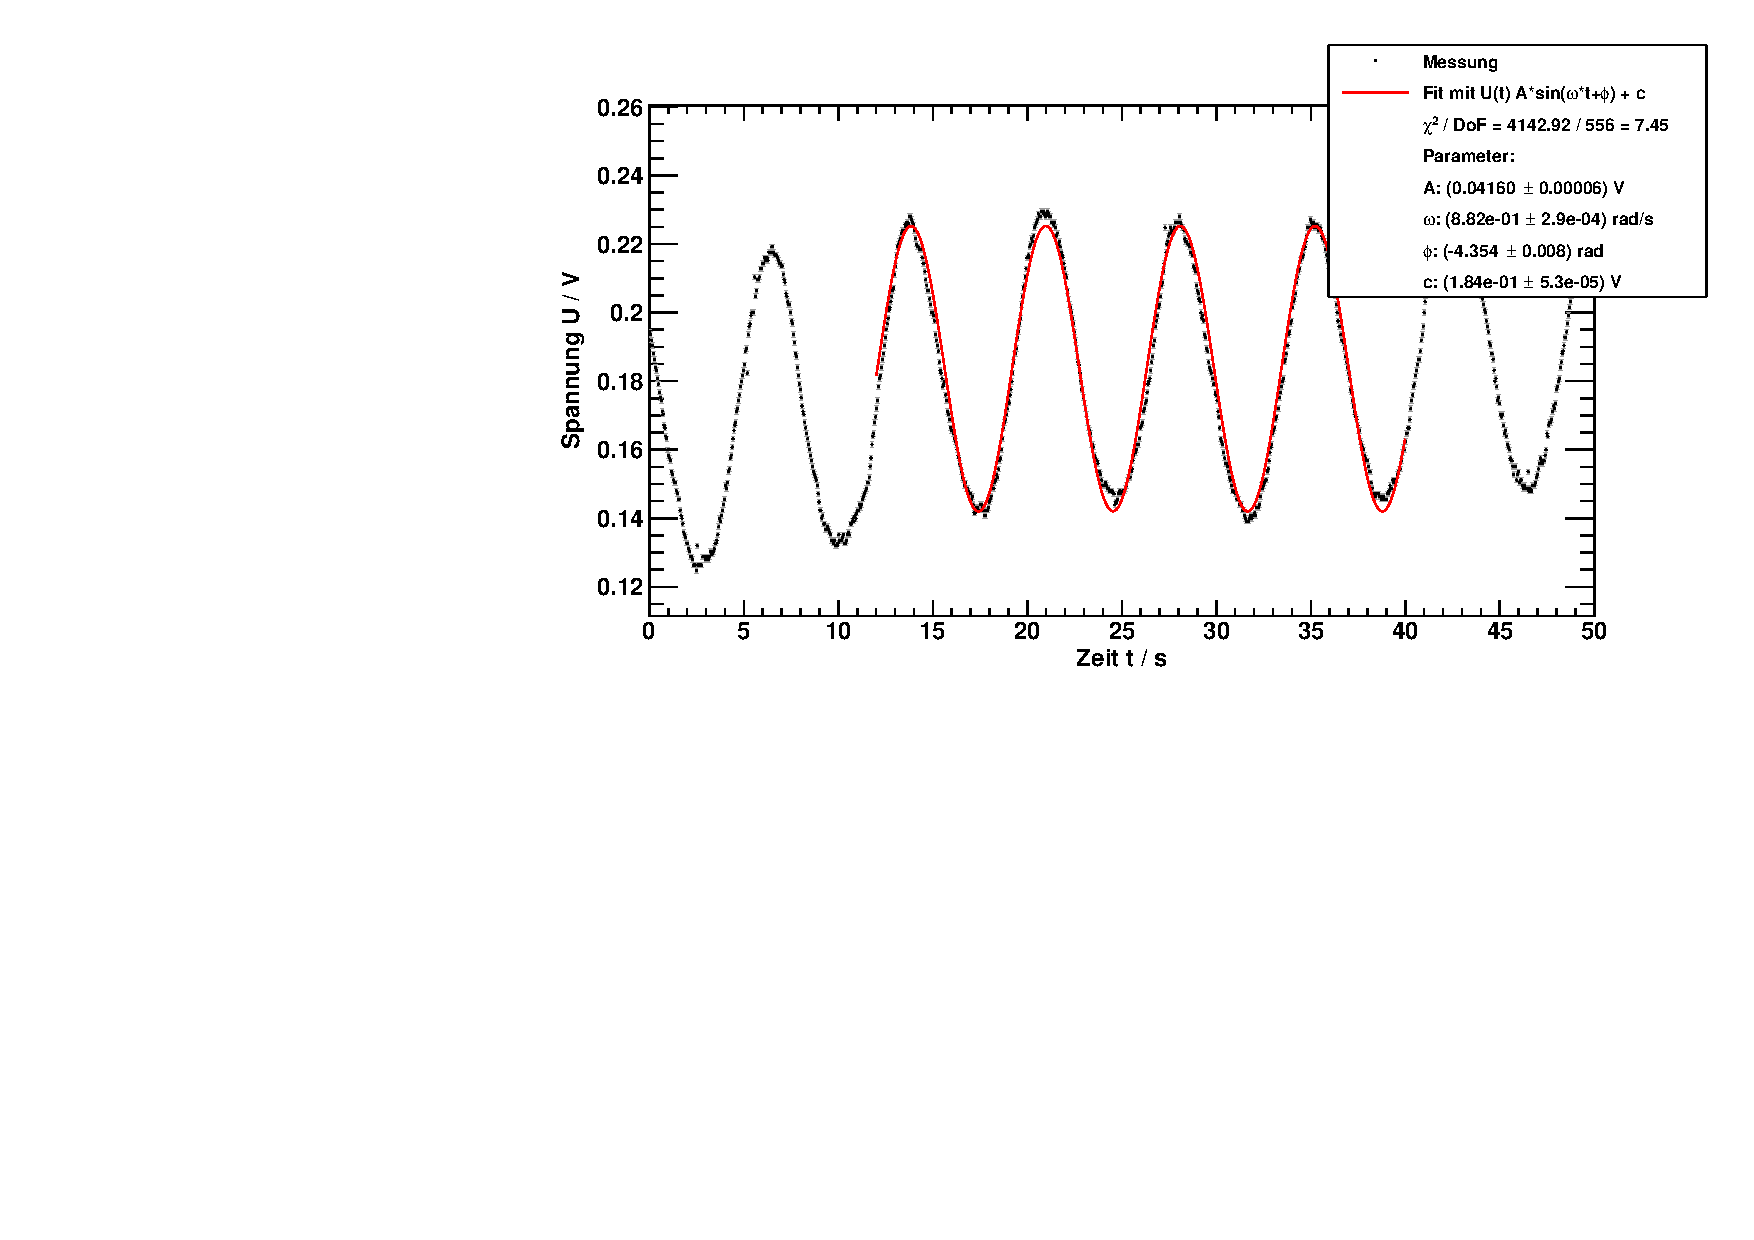
\includegraphics[width=0.64\textwidth]{../img/fit_Spule_R3.pdf}
  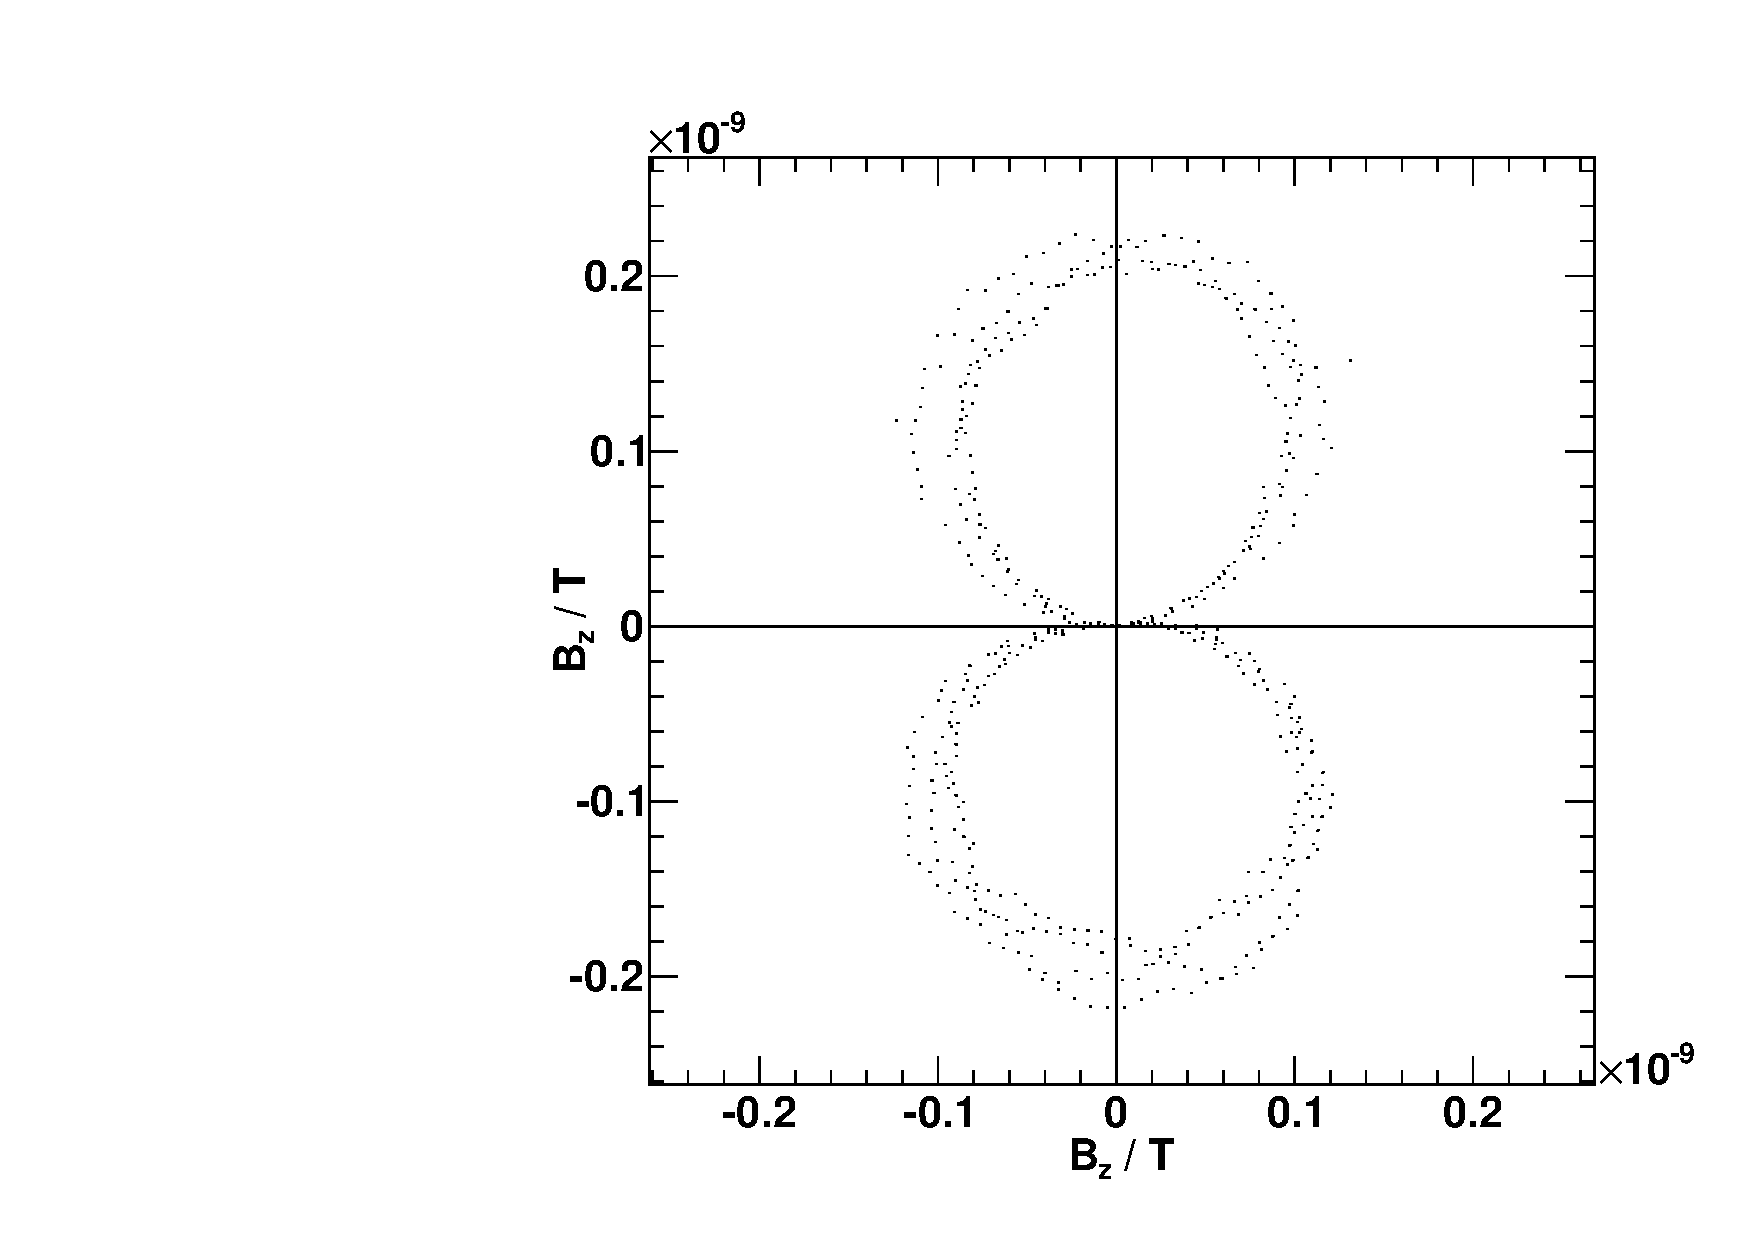
\includegraphics[width=0.35\textwidth]{../img/polar_Spule_R3.pdf}
  \caption{Fit und Polarplot des Magnetfeldes der Leiterschleife mit Widerstand R3.}
  \label{img:R3}
\end{center}
\end{figure}

\begin{figure}[H]
\begin{center}
  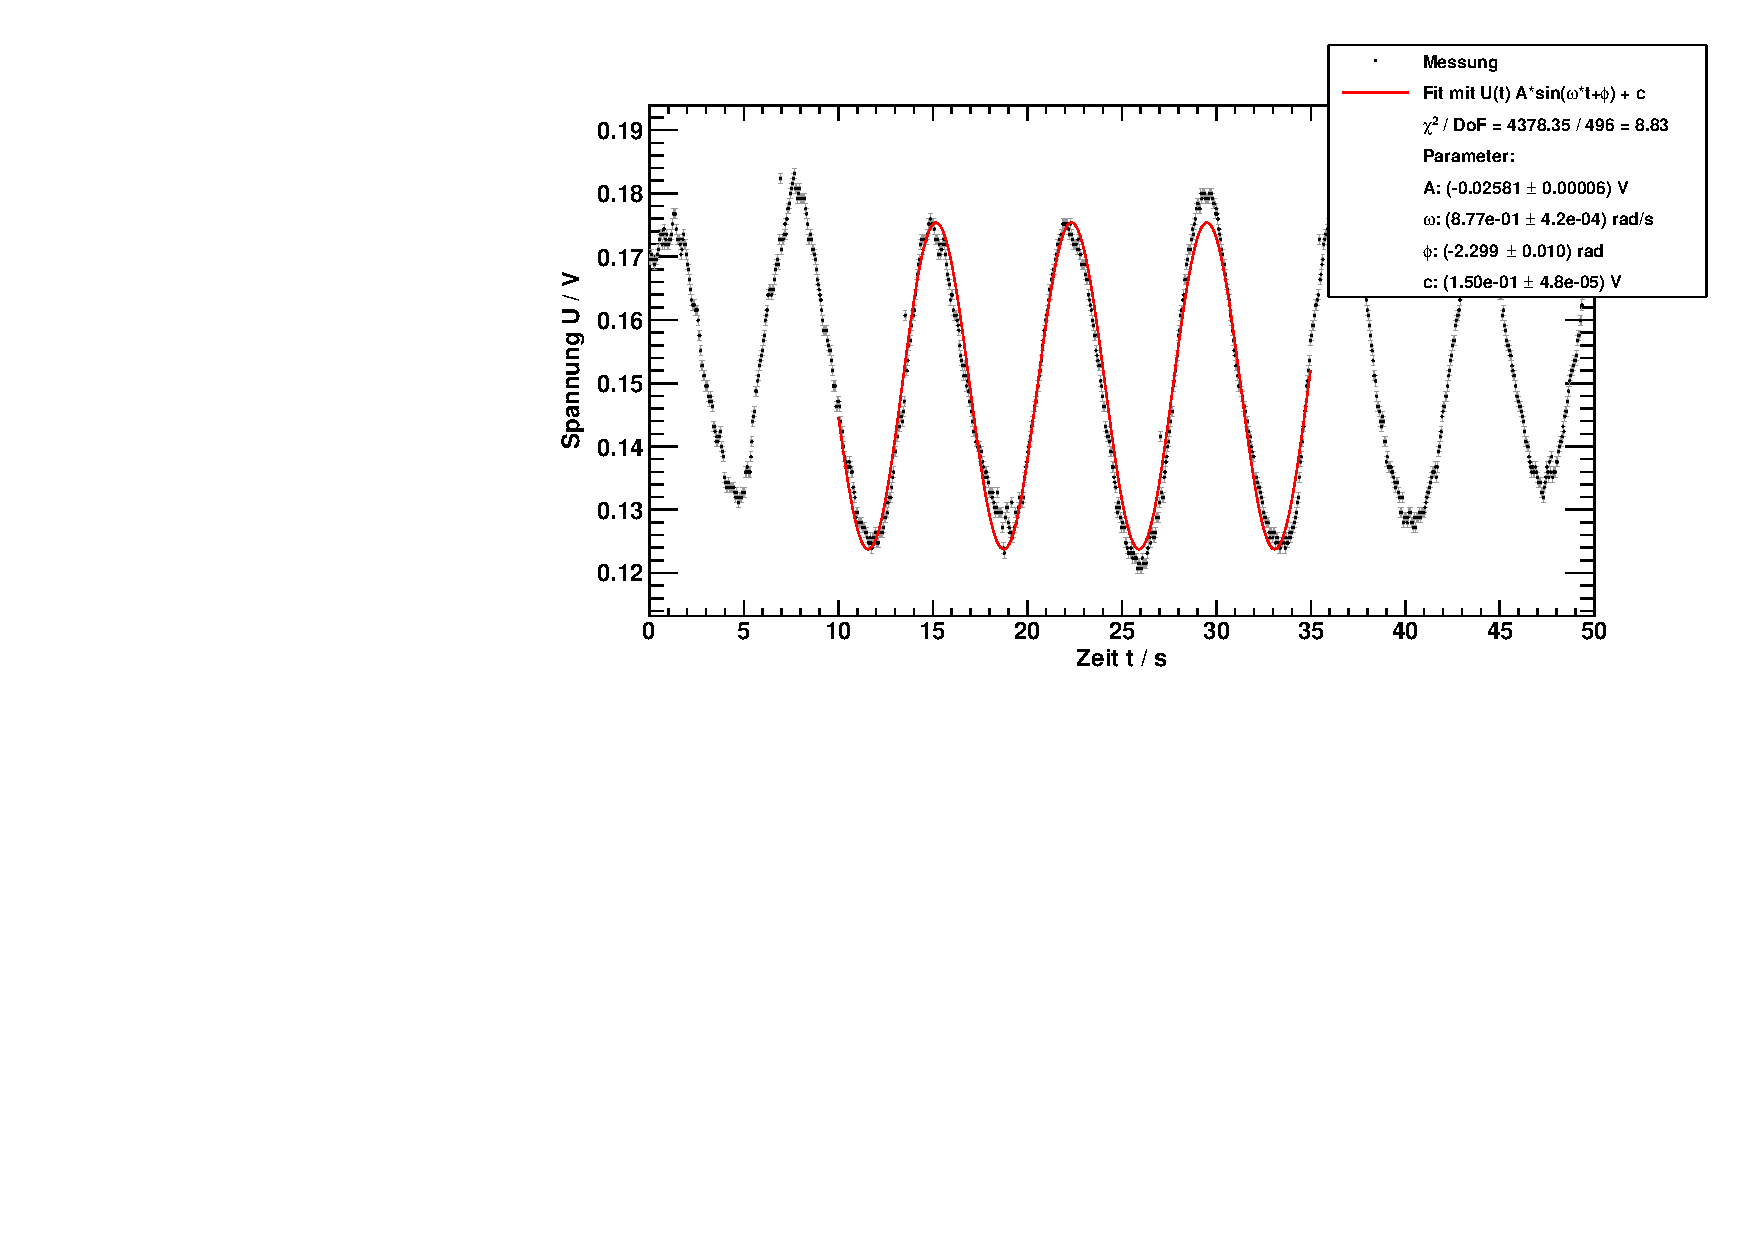
\includegraphics[width=0.64\textwidth]{../img/fit_Spule_R4.pdf}
  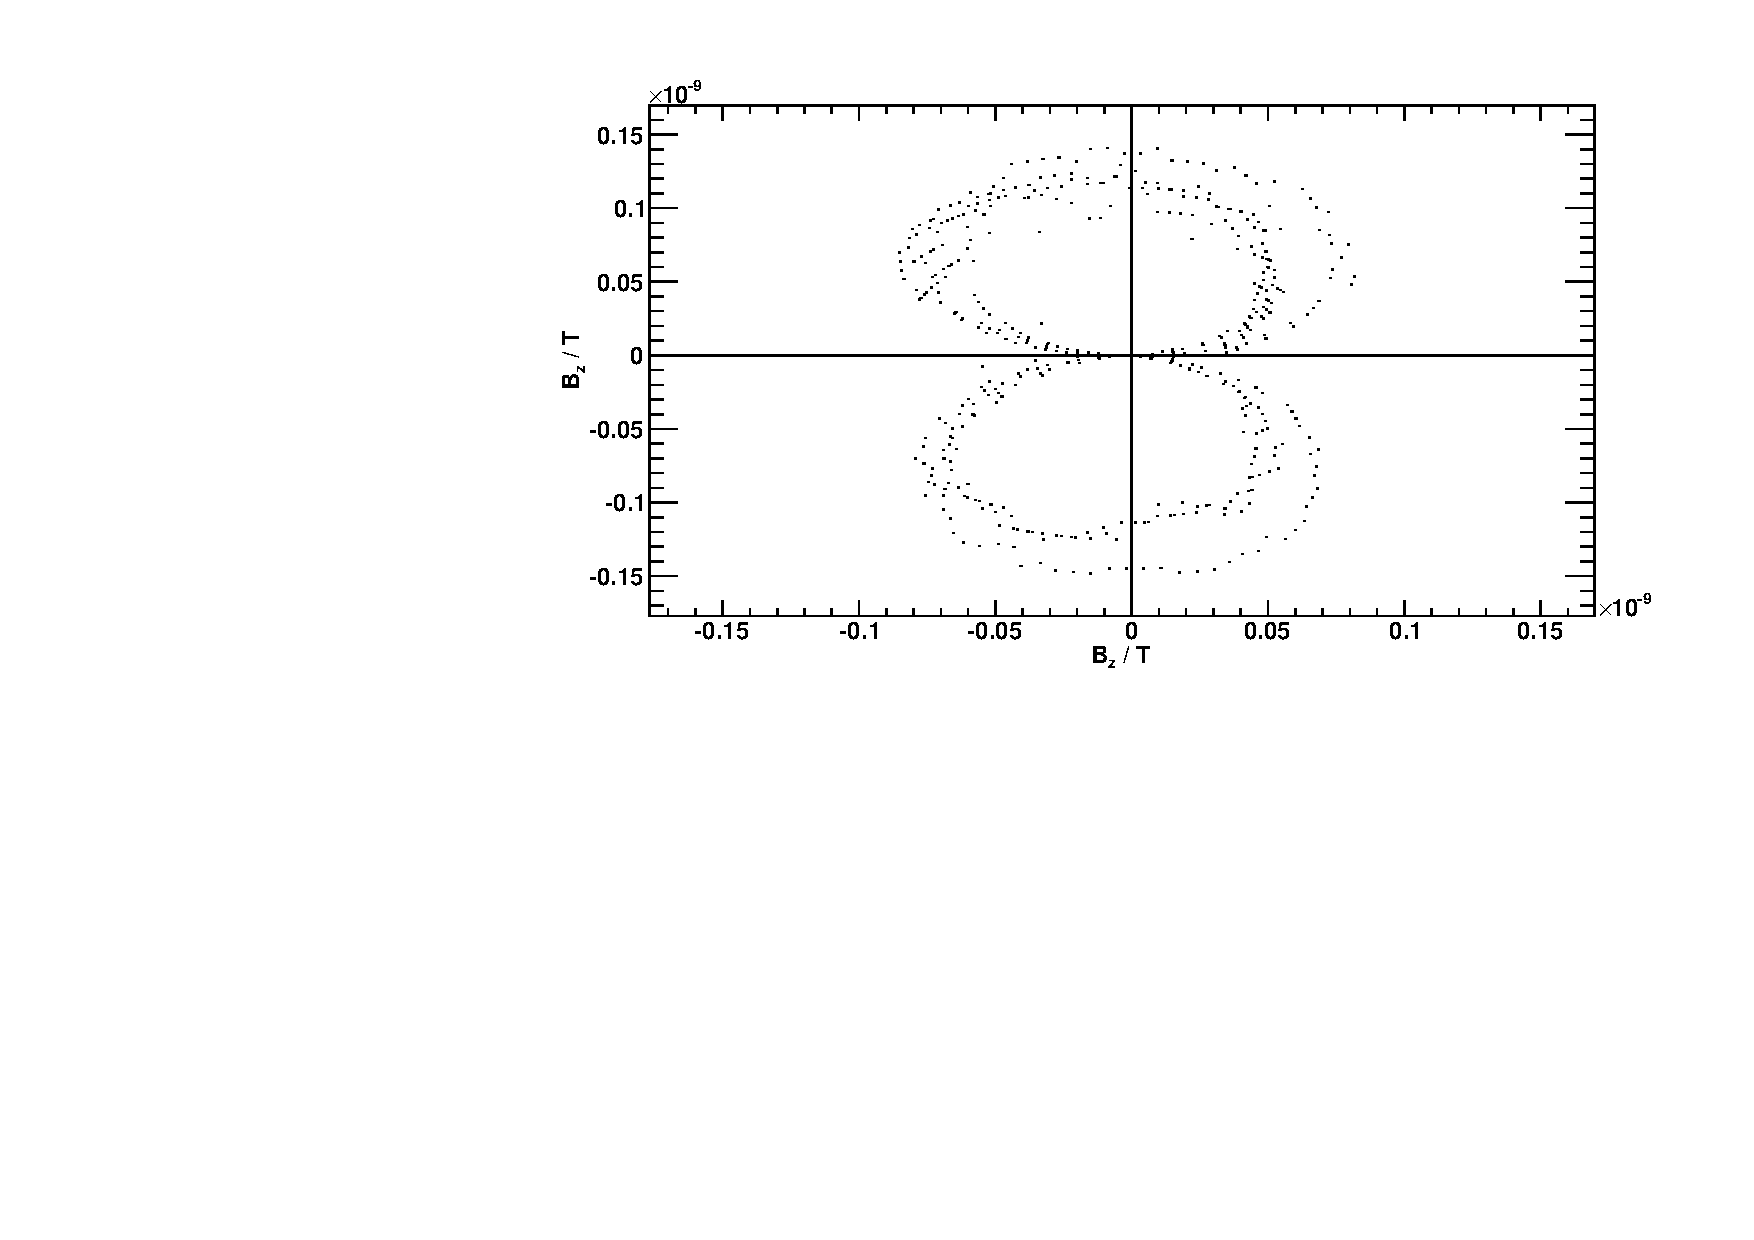
\includegraphics[width=0.35\textwidth]{../img/polar_Spule_R4.pdf}
  \caption{Fit und Polarplot des Magnetfeldes der Leiterschleife mit Widerstand R4.}
  \label{img:R4}
\end{center}
\end{figure}

\begin{figure}[H]
\begin{center}
  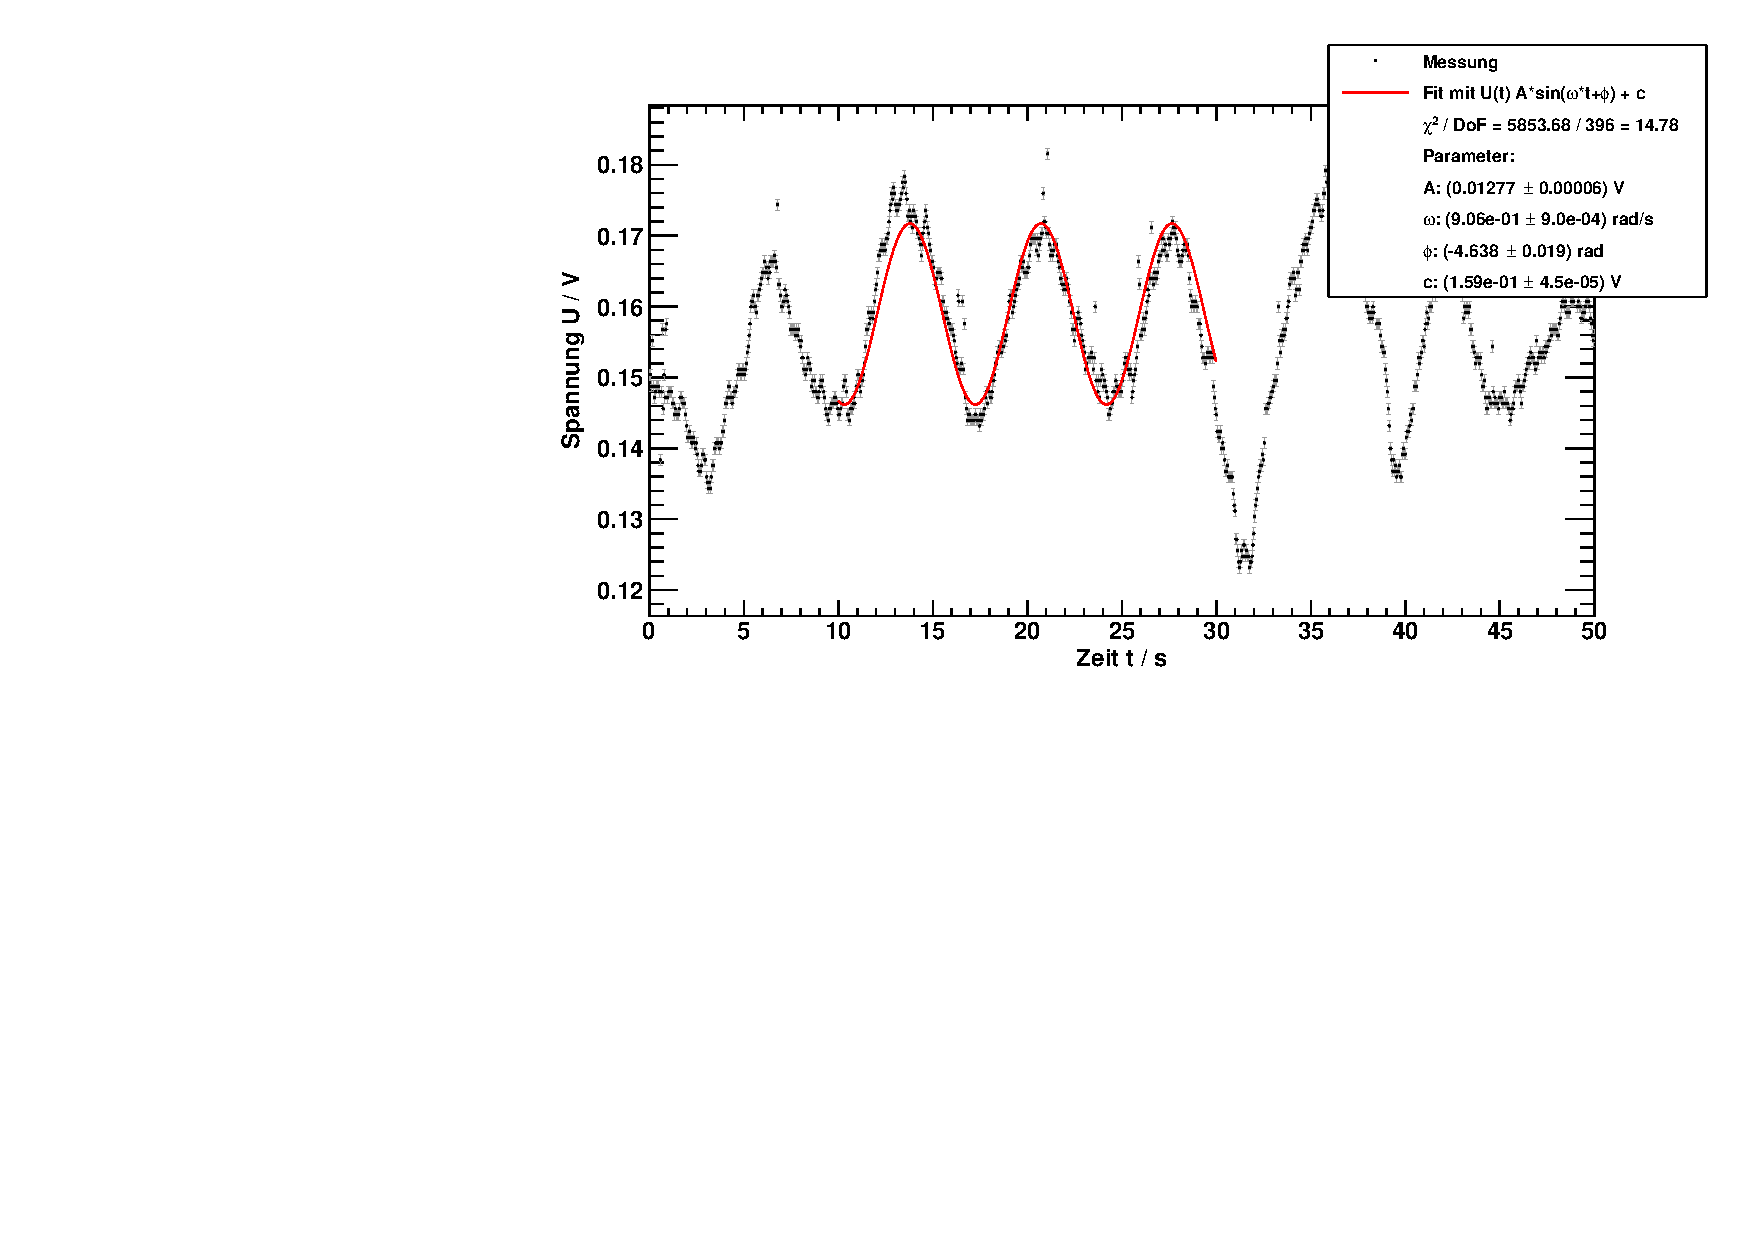
\includegraphics[width=0.64\textwidth]{../img/fit_Spule_R5_1.pdf}
  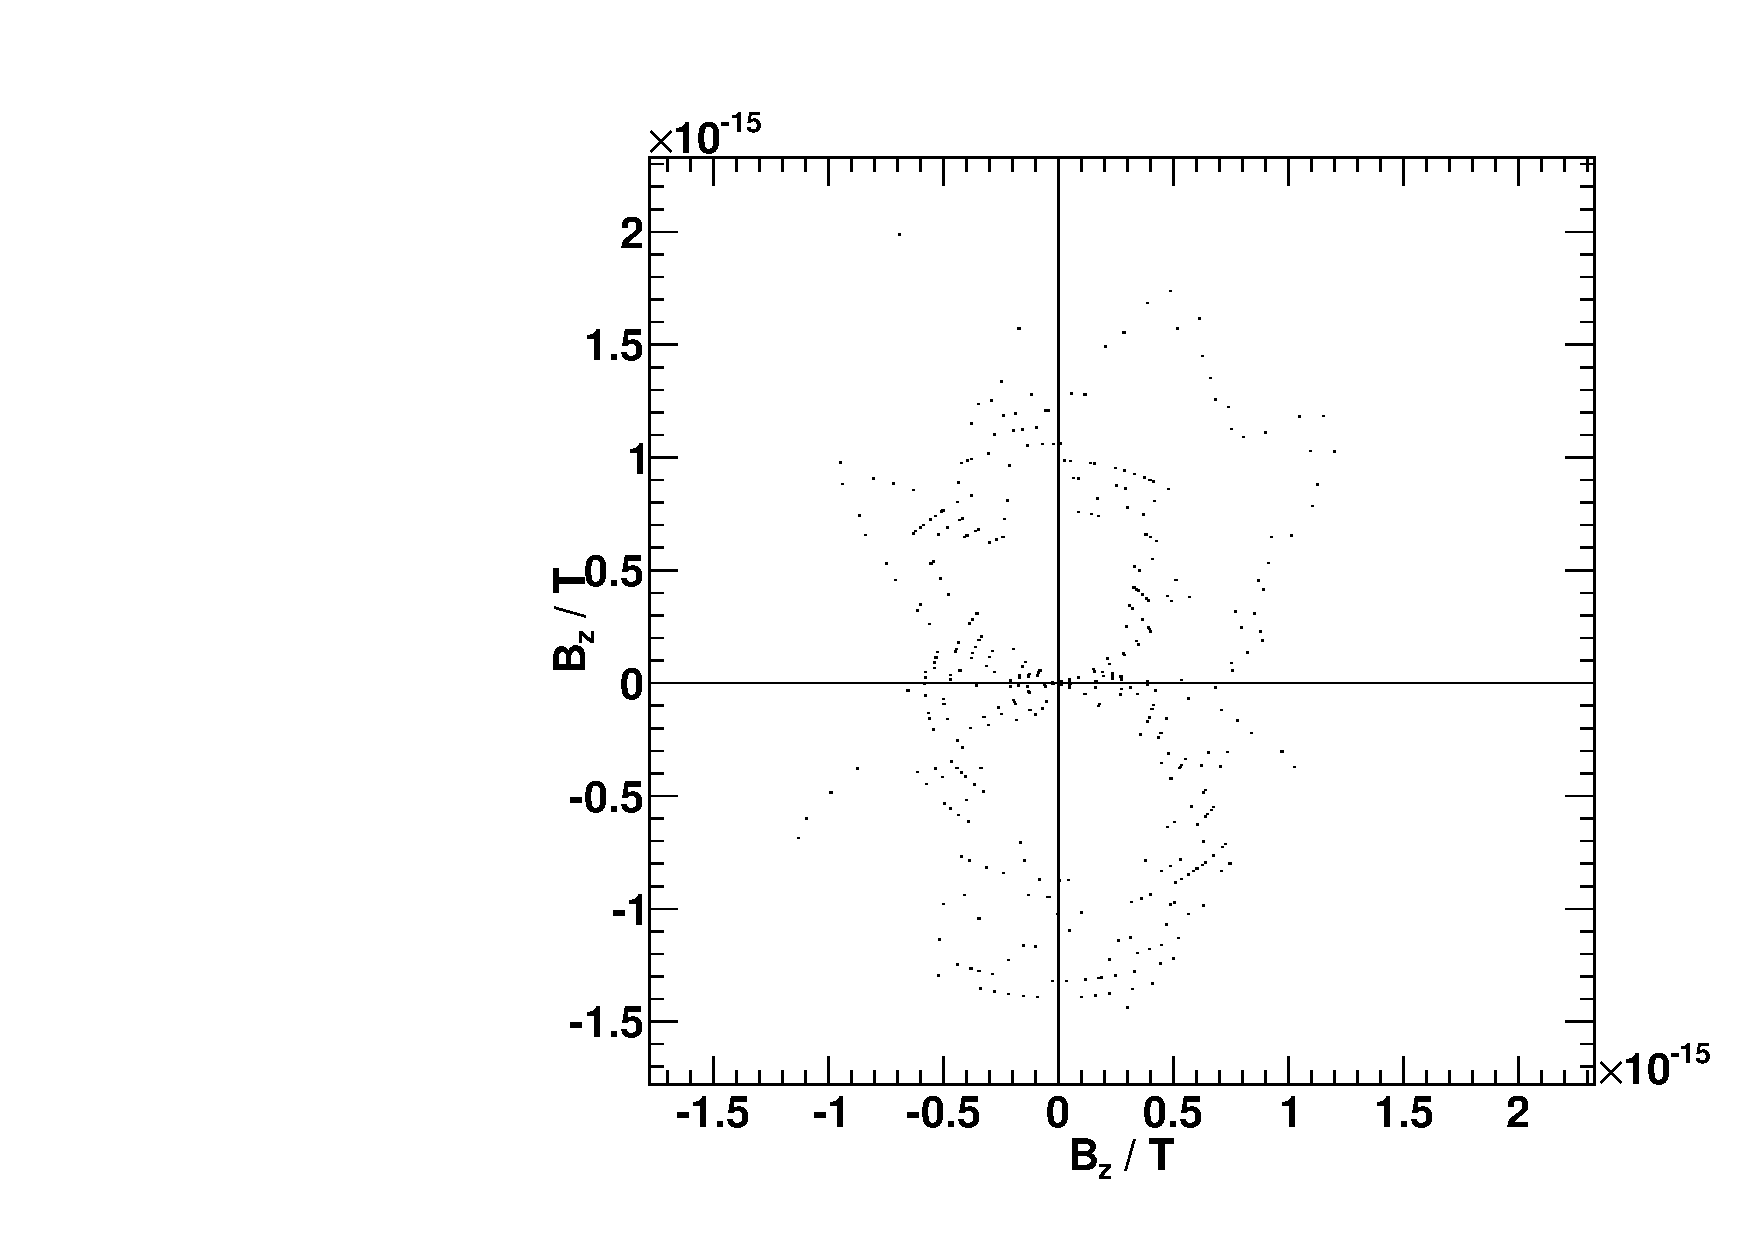
\includegraphics[width=0.35\textwidth]{../img/polar_Spule_R5_1.pdf}
  \caption{Fit und Polarplot des Magnetfeldes der Leiterschleife mit Widerstand R5.}
  \label{img:R5}
\end{center}
\end{figure}

Aus den Amplitude der Fits erhält man mit \autoref{eq:AtoB} die Stärke des Magnetfeldes (\autoref{tab:B:fit}).
\begin{table}[H]
\caption{Gemessene Magnetfeldst"arke $B_z$ in Abh"angigkeit des Widerstandes $R$ der Leiterschleife.}
\begin{center}
\begin{tabular}{|c|c|c|}
  \hline
  $R$ / \textOmega & $B_z$ / nT & $s_{B_z}$ / nT \\ \hline
  100 & 0.57769 & 0.00067 \\ \hline
  510 & 0.30426 & 0.00031 \\ \hline
  1000 & 0.10182 & 0.00015 \\ \hline
  5100 & 0.06317 & 0.00015 \\ \hline
  10000 & 0.03125 & 0.00015 \\ \hline
\end{tabular}
\end{center}
\label{tab:B:fit}
\end{table}

Der Fehler auf $B_z$ ist sehr klein, dies liegt daran, dass er ausschließlich aus den Fehlern der Fitparameter stammt und damit nicht alle 
Fehlermechanismen erfasst werden. Für einen besseren Fehler hätten mehrere Messungen mit den selben Bedingungen durchgeführt werden müssen.

\subsubsection{Berechnung aus der Geometrie der Leiterschleife}
Aus \autoref{eq:Bz:biotsavart} lässt sich nun die theoretische Stärke des Magnetfeldes $B_z$ in $z$-Richtung bestimmen. 
Mit $I = \frac{U}{R}$ und $z'=0$ (Leiterschleife im Ursprung) folgt:
\begin{equation}
  B_z = \frac{\mu \cdot U}{2 R} \cdot \frac{r^2}{ \left( r^2 + z^2 \right)^{3/2}}
\end{equation}
Dabei ist $r$ der Radius, $U$ die angelegte Spannung und $R$ der Widerstand der Leiterschleife. Der Fehler lässt sich mit Gauß'scher 
Fehlerfortpflanzung berechnen:
\begin{equation}
  \begin{split}
     s_{B_z} = \frac{\mu \cdot r}{2 R \left(r^2+z^2\right)^{5/2}} \big( & r^6 \text{sU}^2+r^4 \left(s_r^2 U^2+2 s_U^2 z^2\right) \\ 
     &+r^2 z^2 \left(U^2 \left(9 s_z^2-4 s_r^2\right)+s_U^2 z^2\right)+4 s_r^2 U^2 z^4 \big)^{1/2}
  \end{split}
\end{equation}
Die berechneten Werte sind in \autoref{tab:B:theo} aufgelistet. Der Radius wurde auf $r=(1.90 \pm 0.18)\,$mm und der Abstand auf 
$z=(2.5 \pm 0.3)\,$cm bestimmt.

\begin{table}[H]
\caption{Theoretische Magnetfeldst"arke $B_z$ in Abh"angigkeit des Stroms $I$, der durch die Leiterschleife flie"st.}
\begin{center}
\begin{tabular}{|c|c|c|c|}
  \hline
  $I$ / mA & $s_I$ / mA & $B_z$ / nT & $s_{B_z}$ / nT \\ \hline
  25.0000 & 0.1000 & 3.598 & 1.384 \\ \hline
  4.9804 & 0.0196 & 0.717 & 0.276 \\ \hline
  2.5600 & 0.0100 & 0.368 & 0.142 \\ \hline
  0.5059 & 0.0020 & 0.073 & 0.028 \\ \hline
  0.2600 & 0.0010 & 0.037 & 0.014 \\ \hline
\end{tabular}
\end{center}
\label{tab:B:theo}
\end{table}


\subsubsection{Vergleich gemessener und theoretischer Werte}
Zum Vergleich der mit dem SQUID gemessenen und aus Geometrie der Leiterschleife bestimmten Magnetfeldstärken $B_z$ wurden diese gemeinsam 
in einer doppeltlogarithmischen Graphik über dem Strom $I$ aufgetragen (\autoref{img:compare}). Die Werte stimmen innerhalb des 
maximal 3-$\sigma$-Intervalls überein (vergleiche dazu \autoref{tab:B:fit} und \autoref{tab:B:theo}). Die gemessenen Werte liegen immer unterhalb 
der theoretischen Werte. Dies könnte daran liegen, dass zur Berechnung der theoretischen Werte ein zu kleiner Abstand von SQUID und Leiterschleife 
gemessen wurde.
\begin{figure}[H]
\begin{center}
  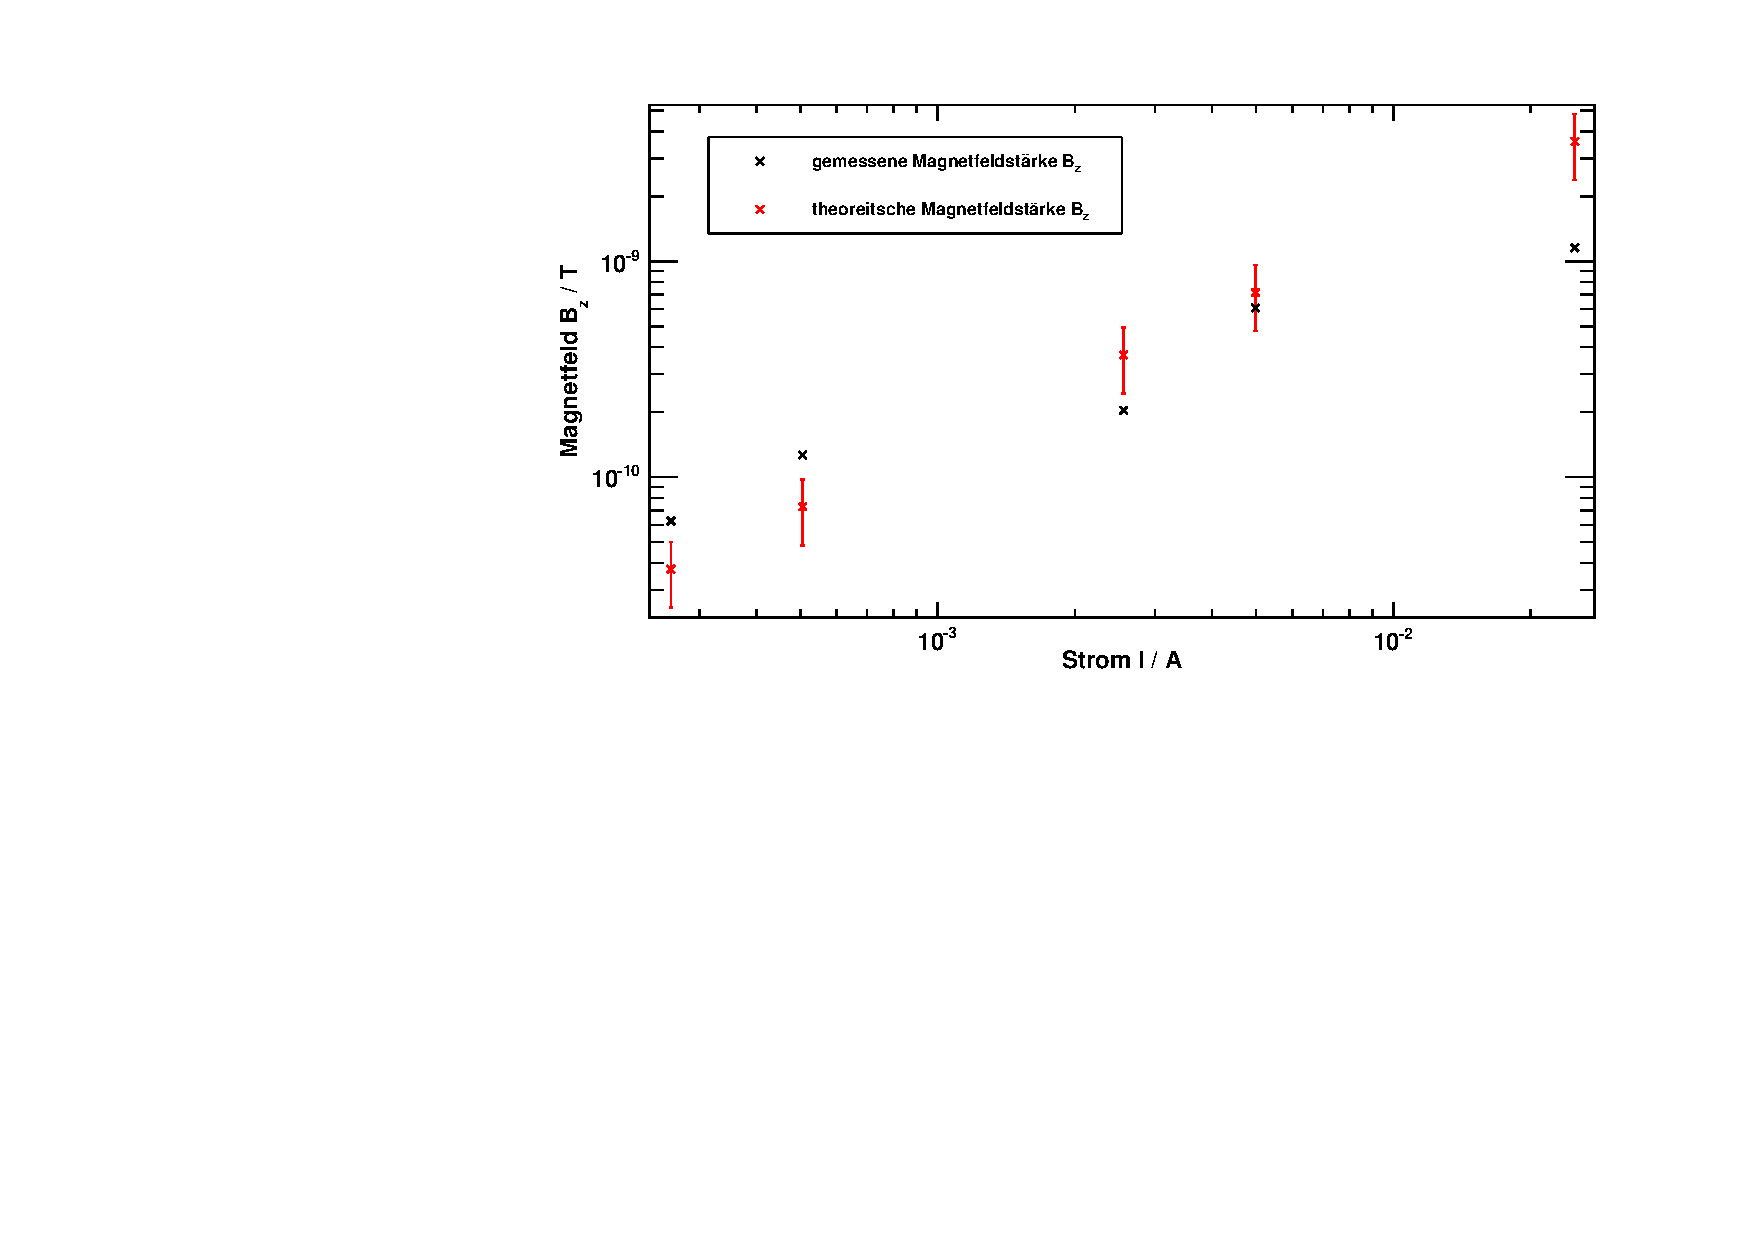
\includegraphics[width=\textwidth]{../img/compare_loglog.pdf}
  \caption{Vergleich von gemessener und theoretischer Magnetfeldstärke $B_z$ der Leiterschleife für verschiedene Ströme $I$.}
  \label{img:compare}
\end{center}
\end{figure}

\subsection{Vermessung des Magnetfelder verschiedener Proben}
Im Folgenden konnten nicht alle SQUID-Signale gefittet werden. Um in diesen Fällen trotzdem einen Polarplot erstellen zu können, wurde der 
Mittelwert aus Kreisfrequenzen der Fits gebildet. Man erhält:
\begin{equation}
  \bar{\omega} = (0.87207 \pm 0.00006) \, \frac{\text{rad}}{\text{s}}
\end{equation}
Der zur Erstellung der Polarplots nötige y-Offset der Daten wurde mit dem Mittelwert aller Messpunkte genähert. Dies ist vertretbar, da es sich 
um periodische Signale handelt.

\subsubsection{Untergrund}
\autoref{img:underground} zeigt das \emph{SQUID}-Signal bei ausgeschaltetem Motor, ohne Probe.
Es ist keine Periodizität des Signals zu erkennen. Die Schwankungen sind statistisch
und werden vermutlich durch wechselnde Magnetfelder von elektrischen Verbrauchern in der Umgebung verursacht.
Ein derartiges Untergrundrauschen mit 10\,mV bis 20\,mV Amplitude
ist allen Messungen überlagert und führt bei geringen Signalamplituden zu
Deformation und Drift der Messsignale.

\begin{figure}[H]
\begin{center}
  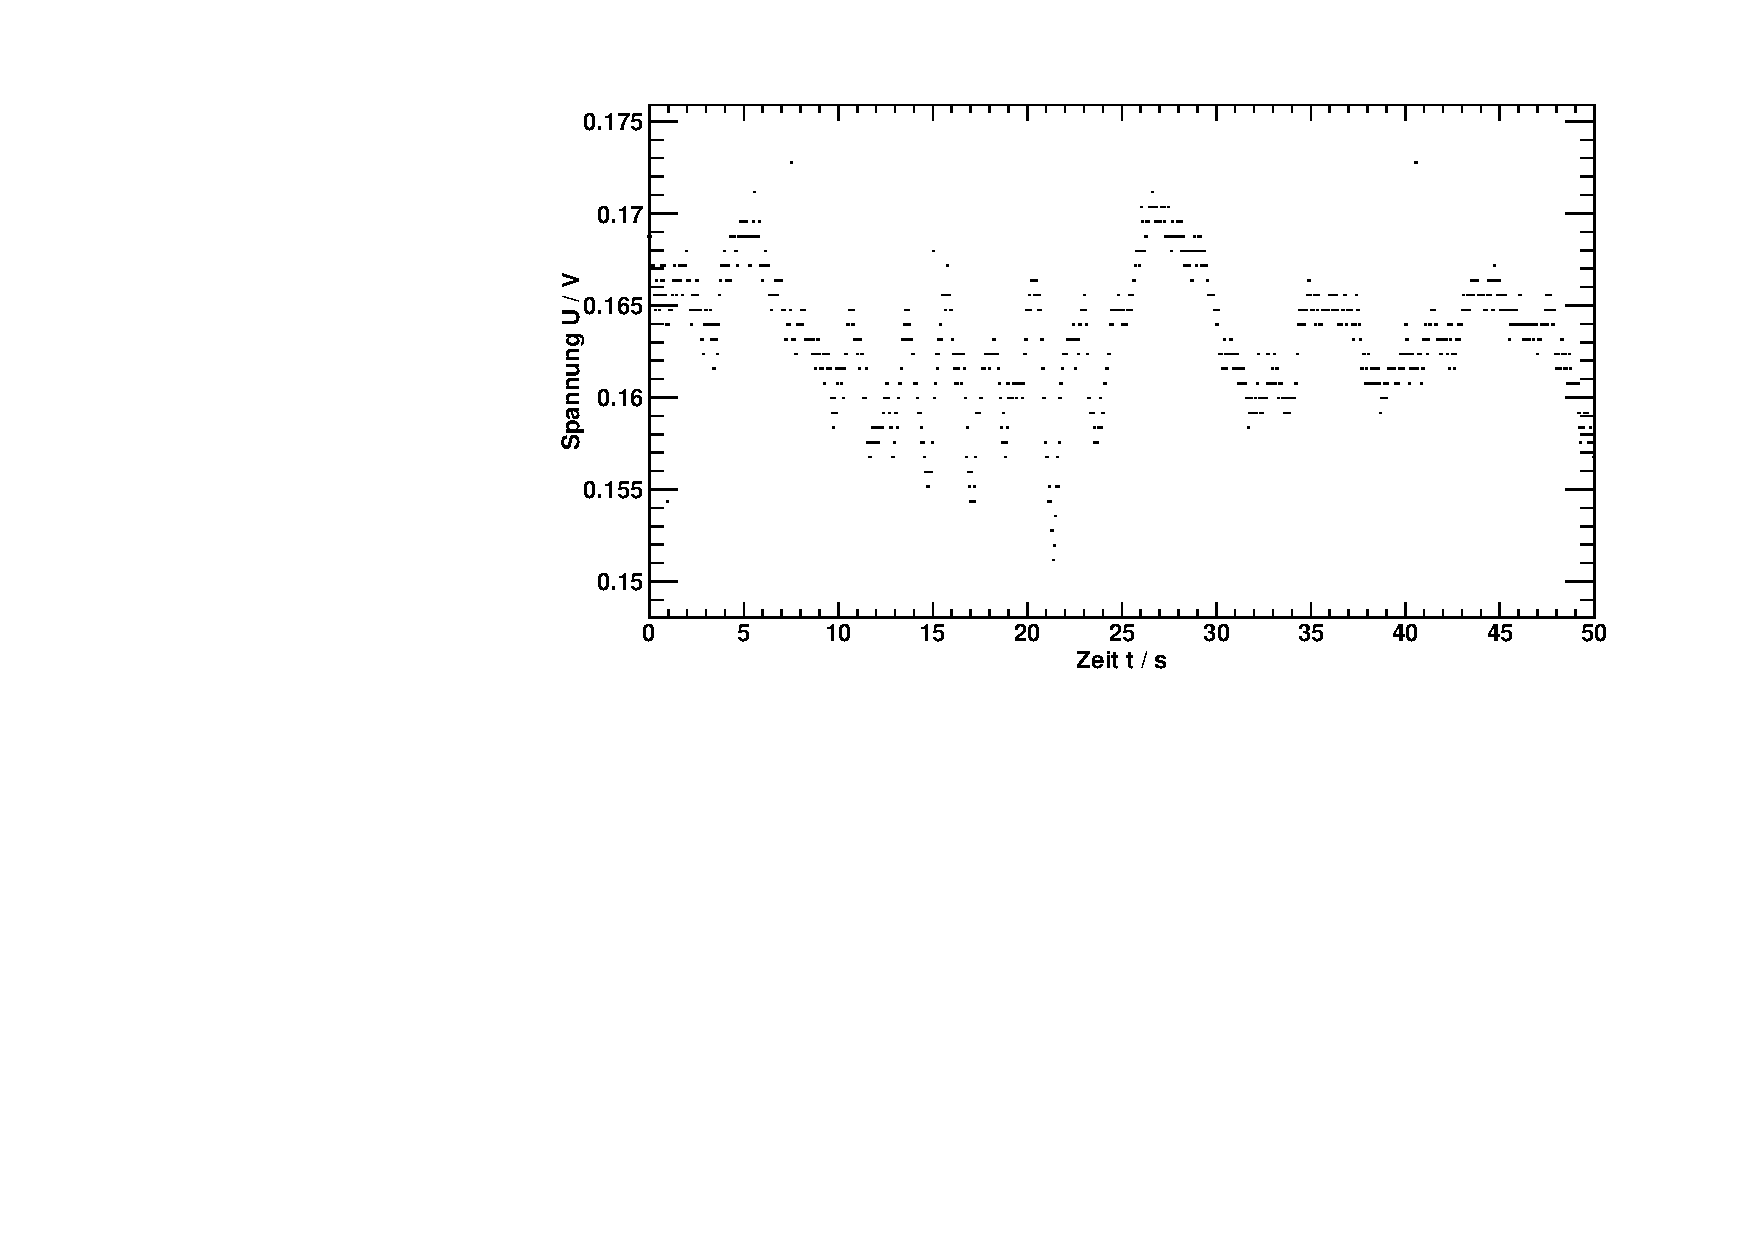
\includegraphics[width=0.8\textwidth]{../img/Untergrund.pdf}
  \caption{\emph{SQUID}-Signal ohne Probe, bei ausgeschaltetem Motor.}
  \label{img:underground}
\end{center}
\end{figure}

\subsubsection{Probenhalter}
Eine weitere Untergrundmessung ohne Probe wurde mit rotierendem Proben\-hal\-ter durch\-ge\-führt.
Hier wird ein periodisches Signal mit ca. 40\,mV Amplitude gemessen.
Der Probenhalter ist also leicht magnetisch.\\
Zur Erstellung des Polarplots wurde der Mittelwert über die Winkelgeschwindigkeiten gebildet,
die aus den Sinusfits gewonnen wurden.
Im Polarplot ist keine deutliche Winkelabhängigkeit zu erkennen.

\begin{figure}[H]
\begin{center}
  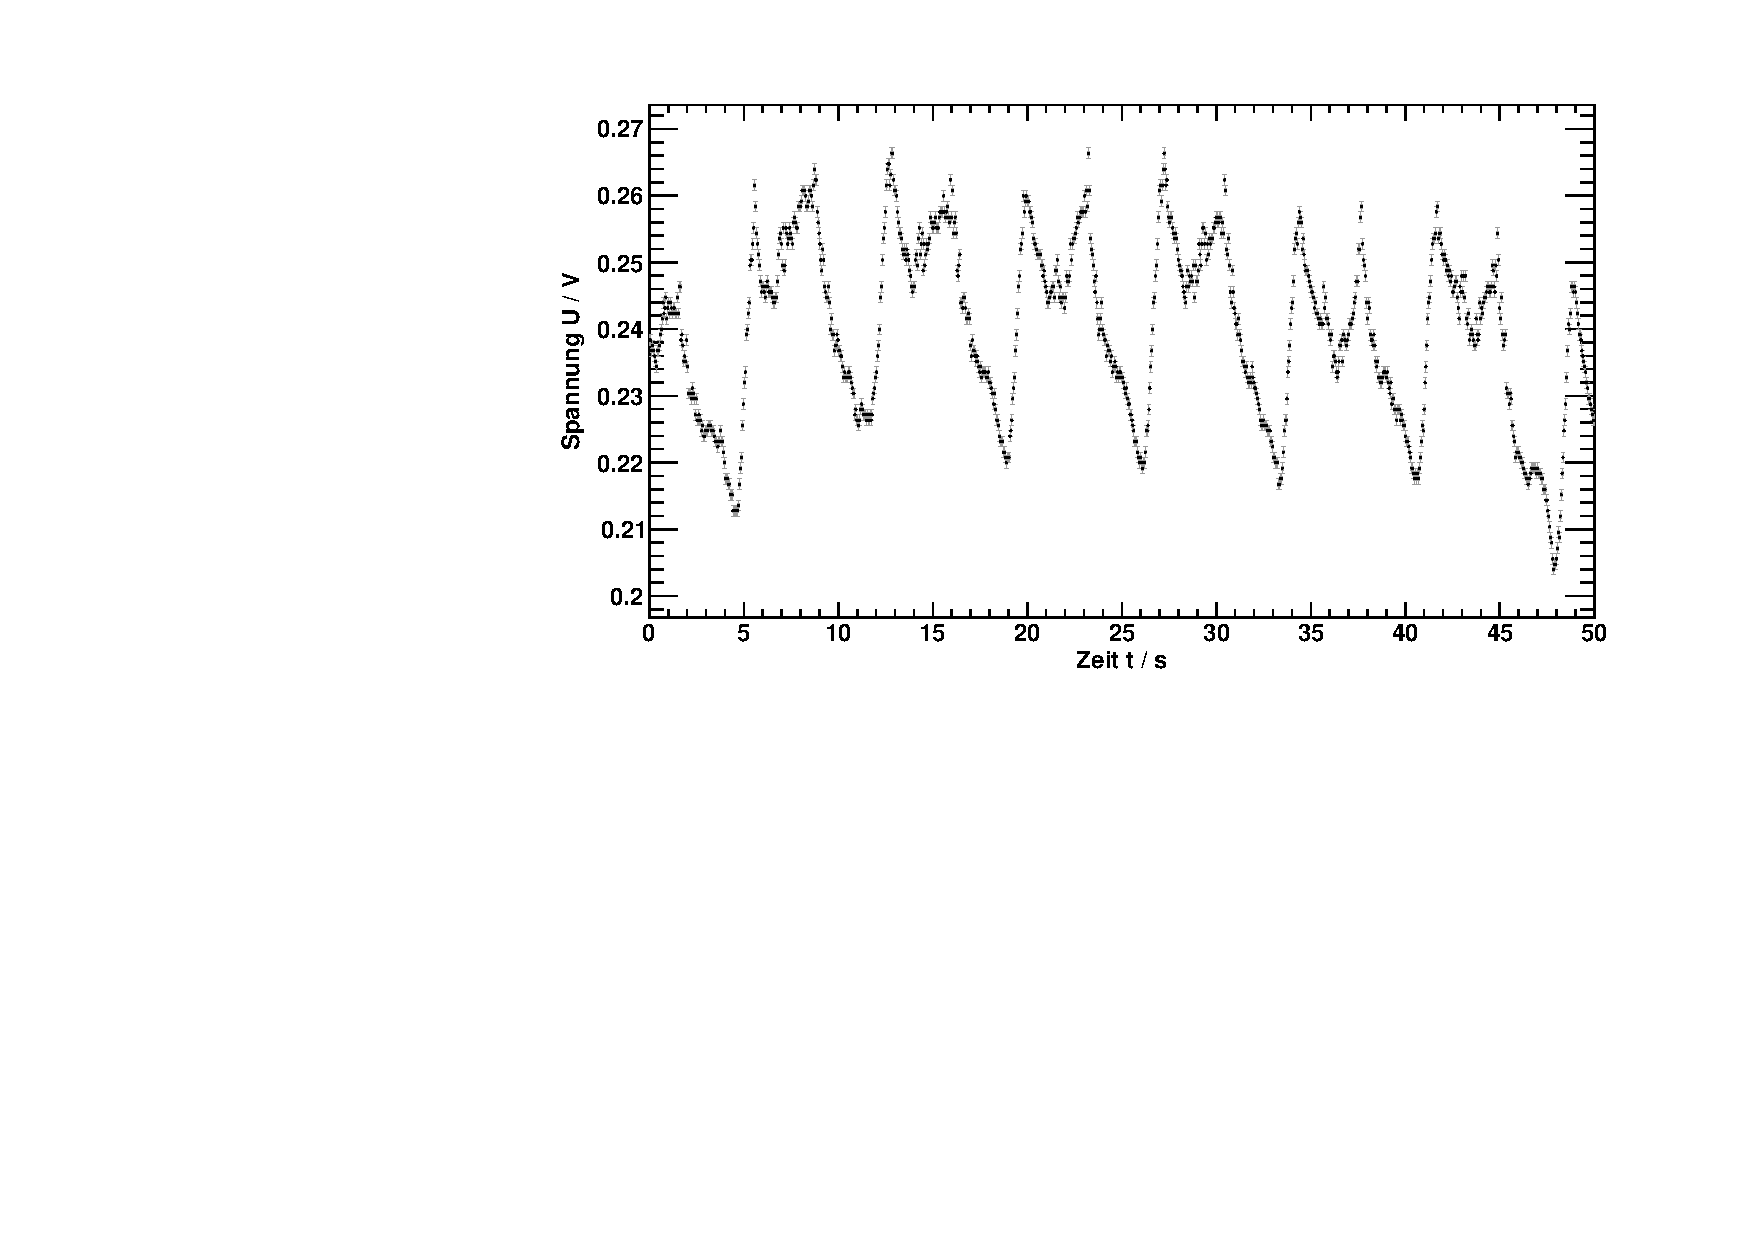
\includegraphics[width=0.64\textwidth]{../img/emptyHolder.pdf}
  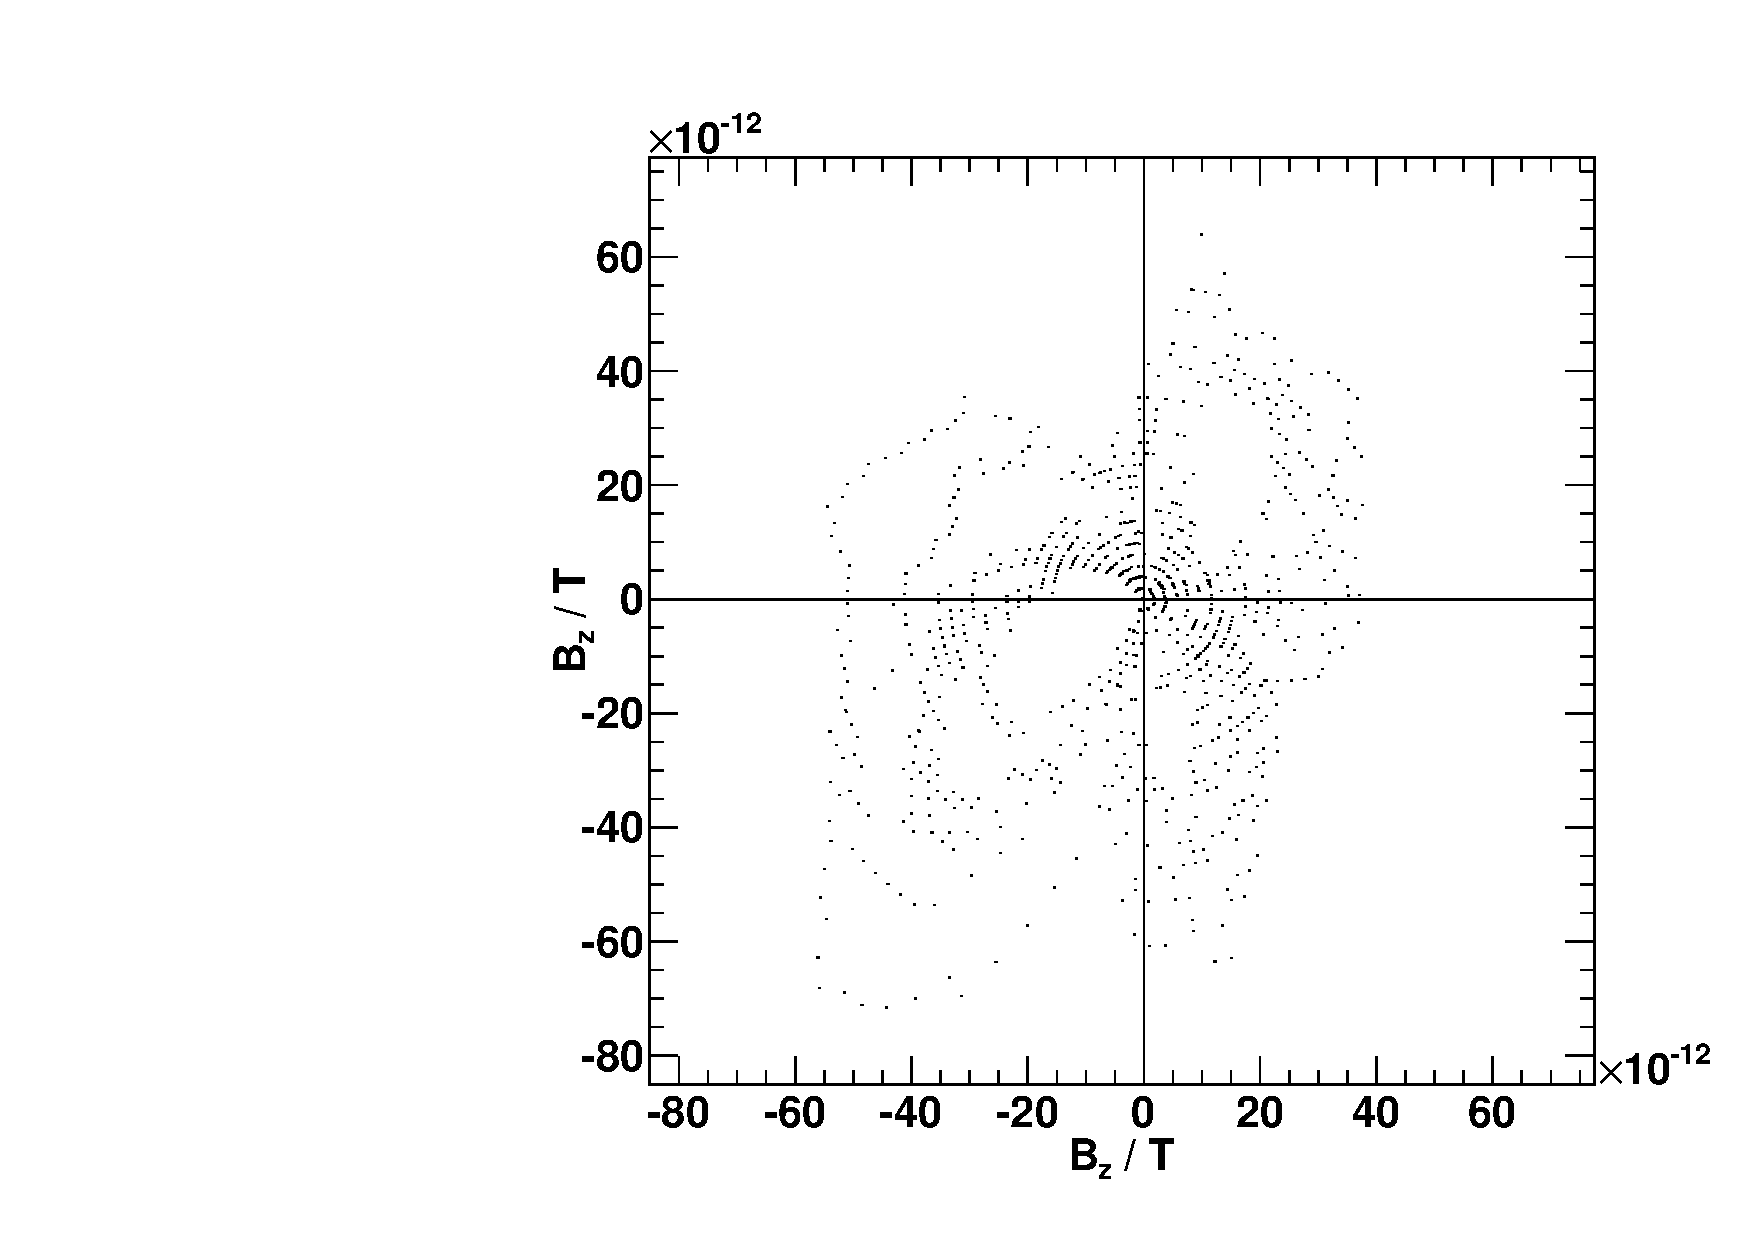
\includegraphics[width=0.35\textwidth]{../img/polar_emptyHolder.pdf}
  \caption{\emph{SQUID}-Signal bei leerem, rotierendem Probenhalter. Es ist eine leichte Magnetisierung des
  Probenhalters erkennbar.}
  \label{img:holder}
\end{center}
\end{figure}

\subsubsection{Stabmagnet}
\begin{figure}[H]
\begin{center}
  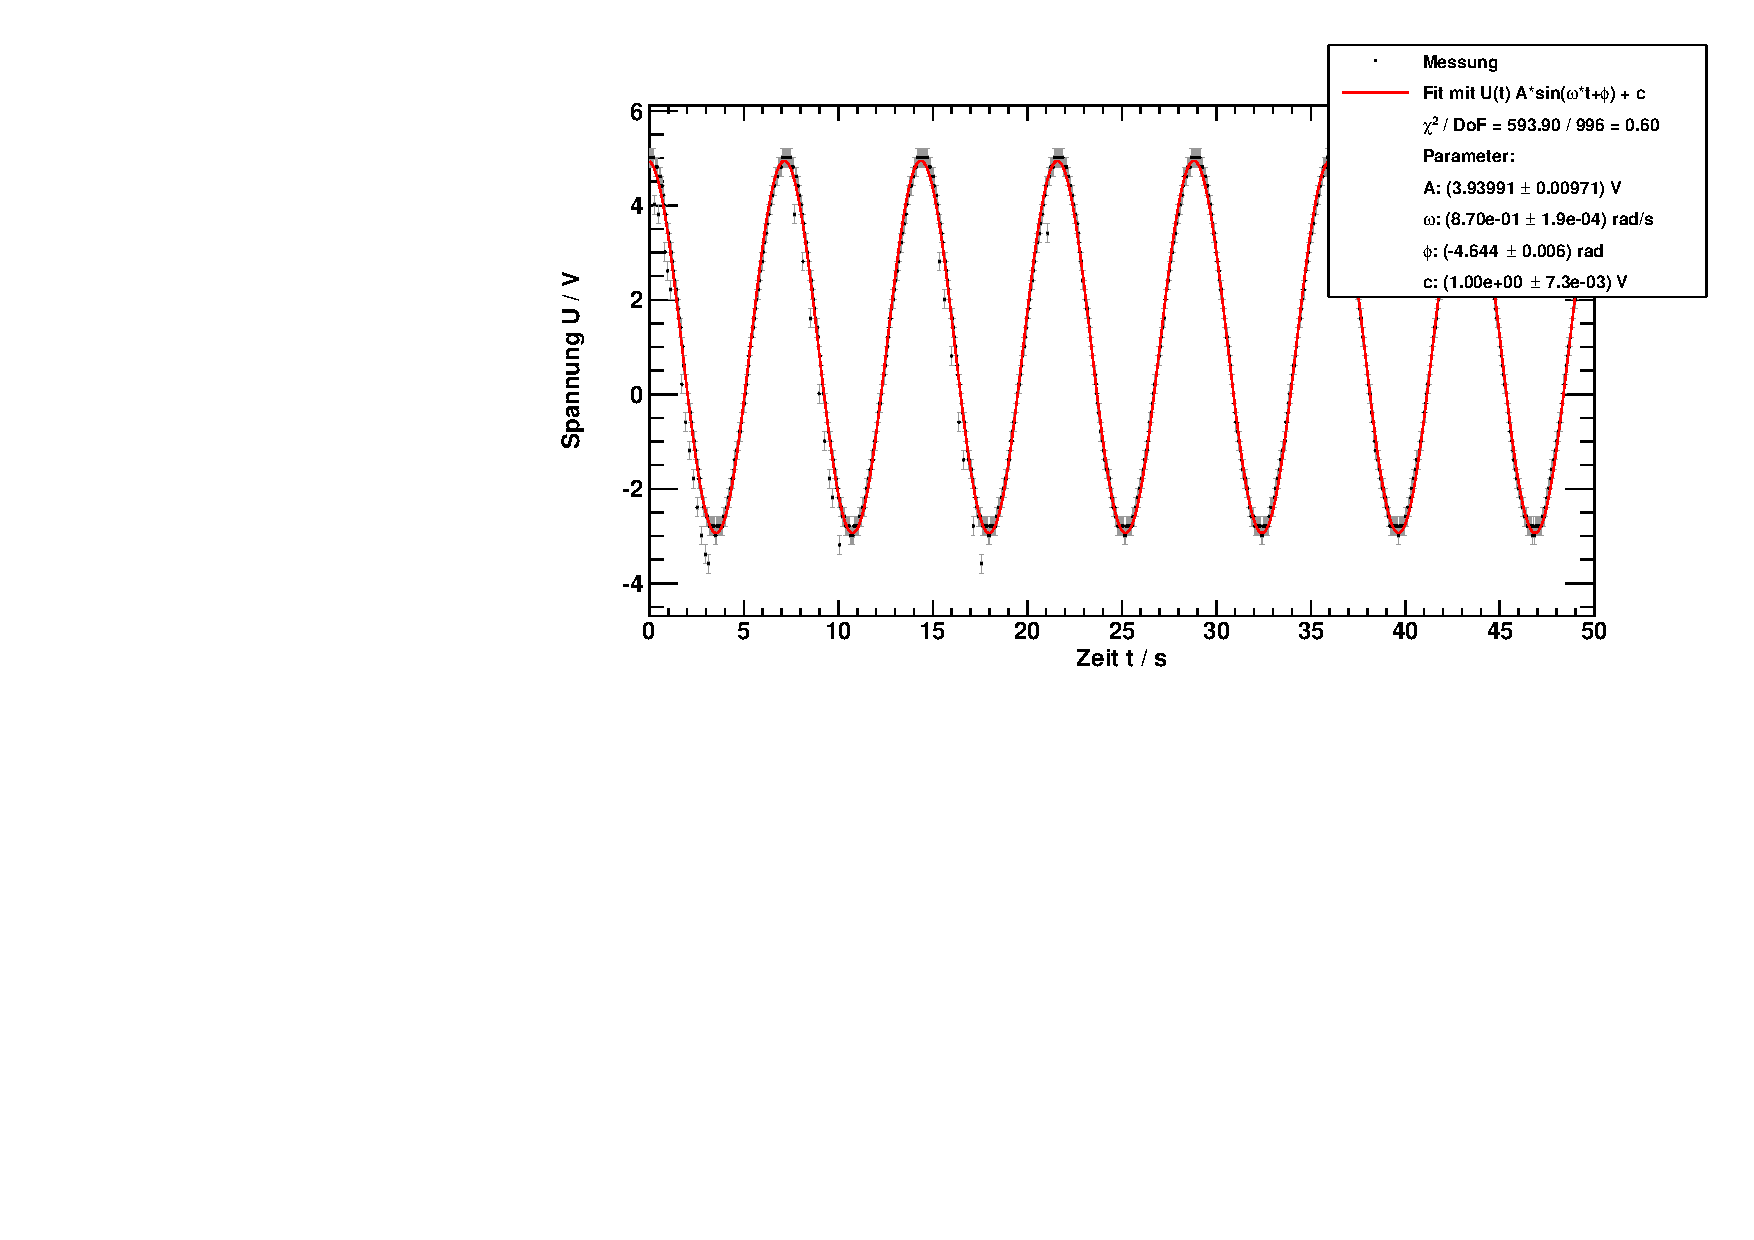
\includegraphics[width=0.64\textwidth]{../img/fit_Magnet.pdf}
  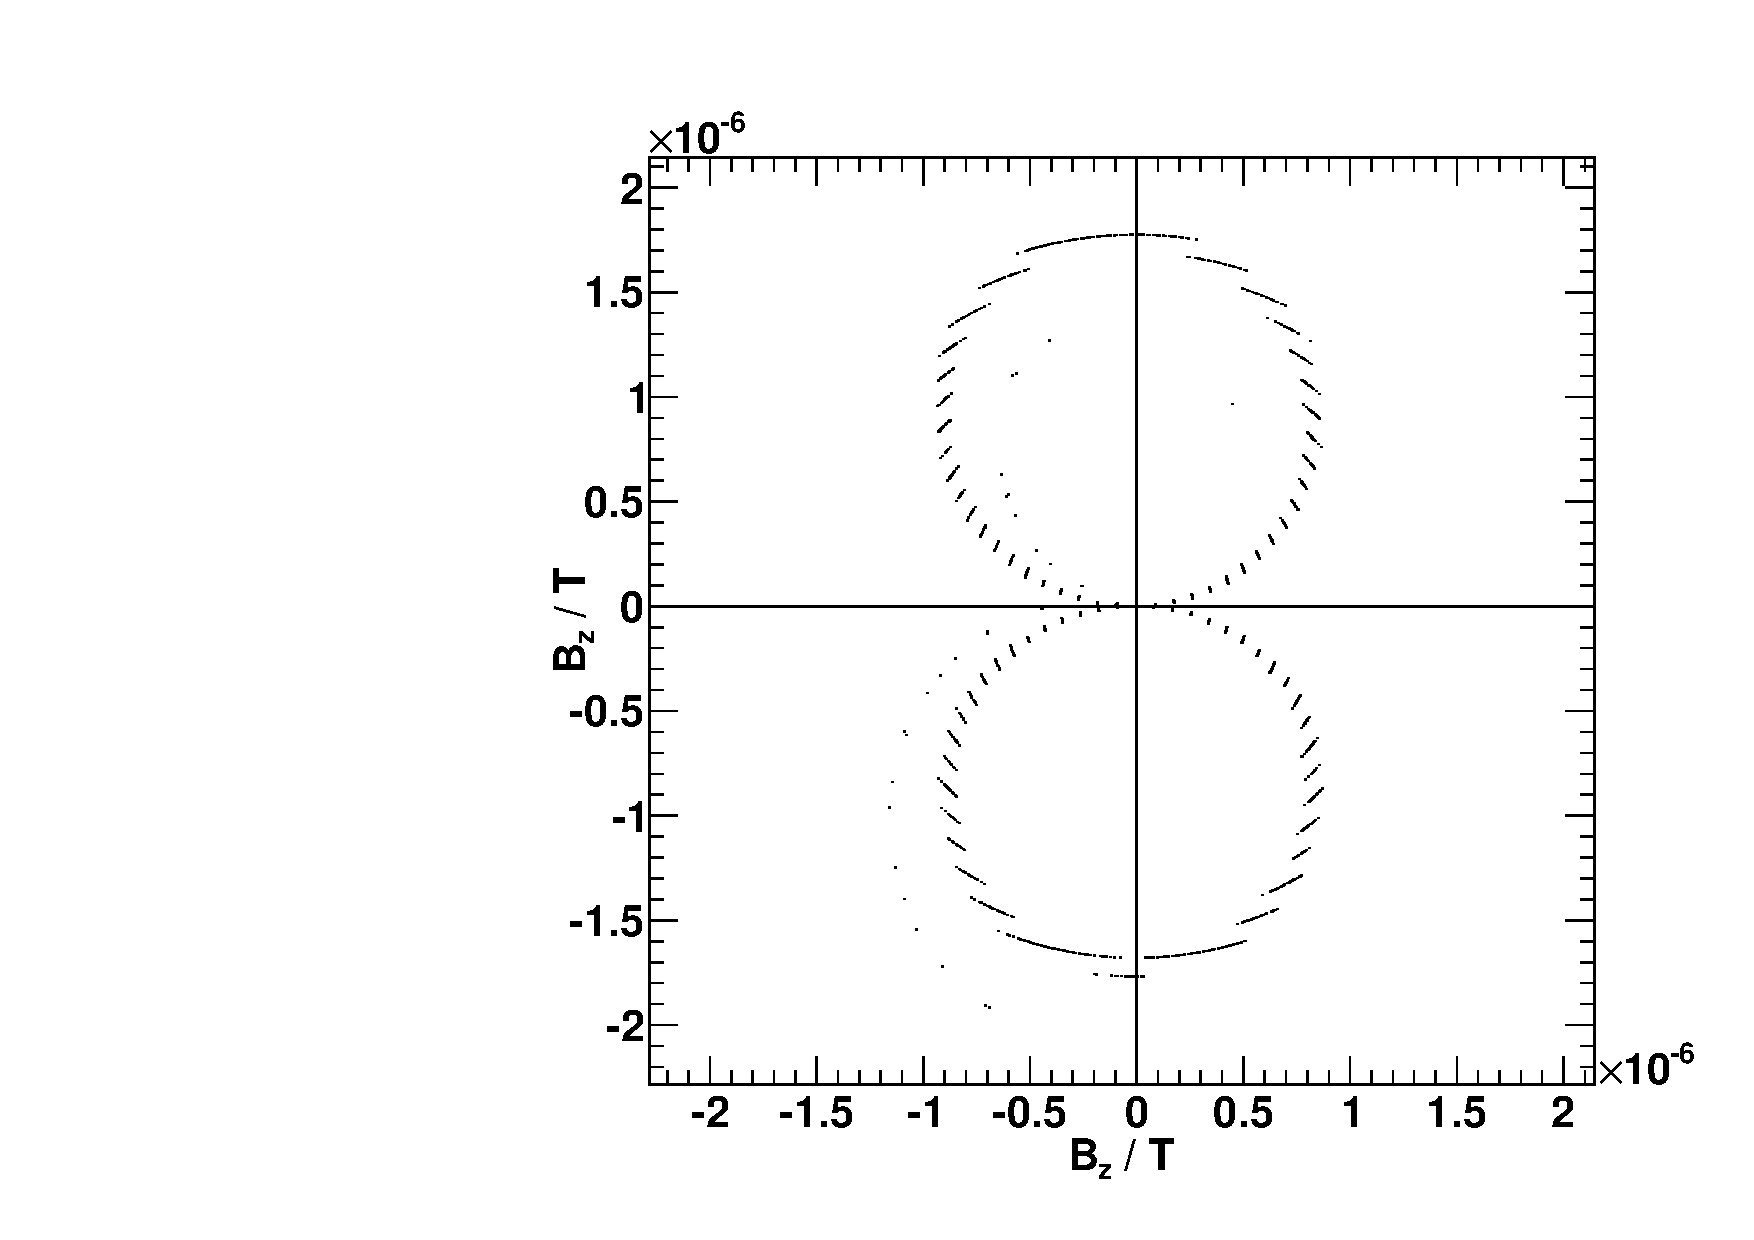
\includegraphics[width=0.35\textwidth]{../img/polar_Magnet.pdf}
  \caption{Bestimmung des Magnetfelds eines kleinen Stabmagneten und Fit mit Sinusfunktion.}
  \label{img:magnet}
\end{center}
\end{figure}
Die Messung am Stabmagneten wurde gemäß \autoref{eq:fit} gefittet.
Für die Amplitude der Schwingung erhält man
\begin{equation}
A_{\text{St}}=(3.9399 \pm 0.0010)\, \text{V} \ \, .
\end{equation}
Daraus folgt nach \autoref{eq:AtoB} für die maximale Magnetfeldstärke des Stabmagneten
\begin{equation}
B_{\text{St}} = (872 \pm 2)\,\text{nT} \ \, .
\end{equation}
Auf dem Polarplot ist deutlich die Struktur des magnetischen Dipols zu erkennen.


\subsubsection{Magnetspan}
\begin{figure}[H]
\begin{center}
  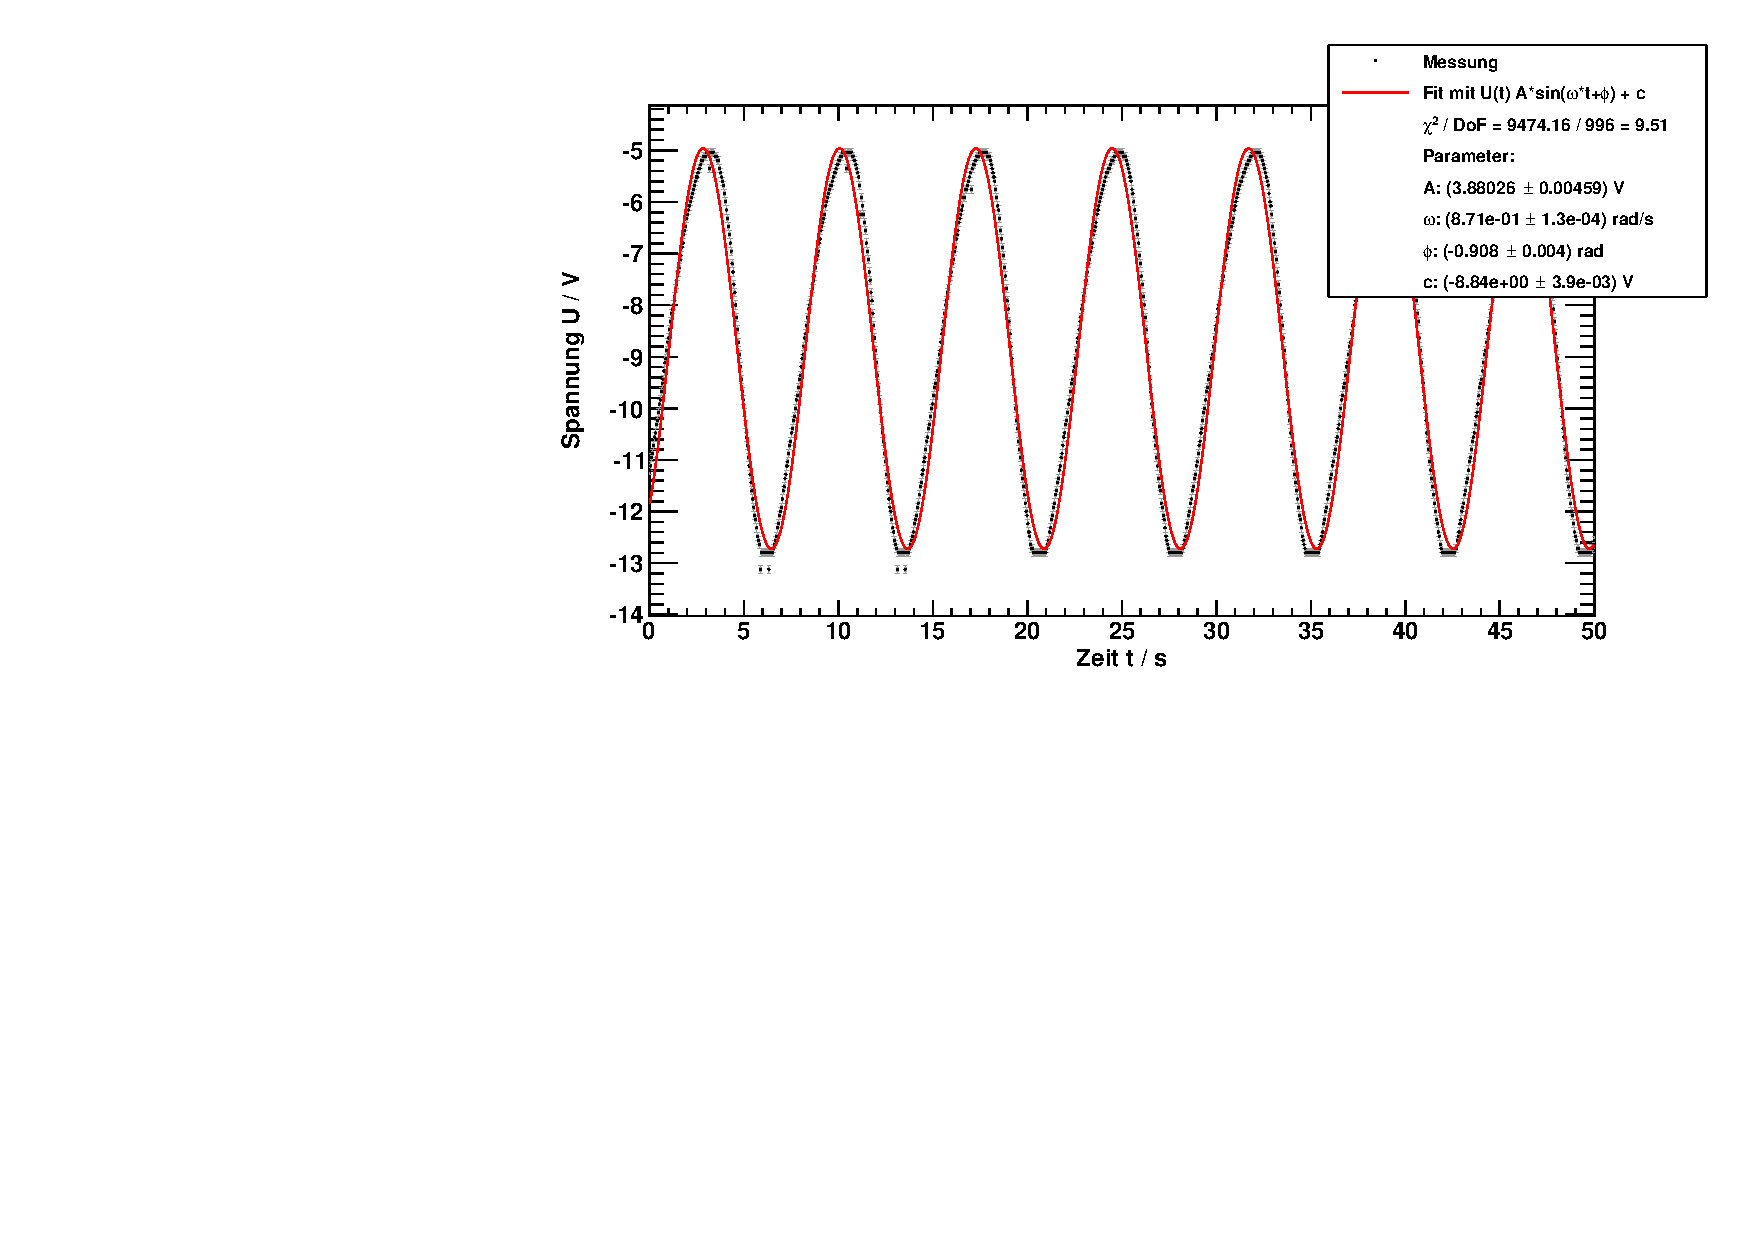
\includegraphics[width=0.64\textwidth]{../img/fit_Magnetspan_45grad.pdf}
  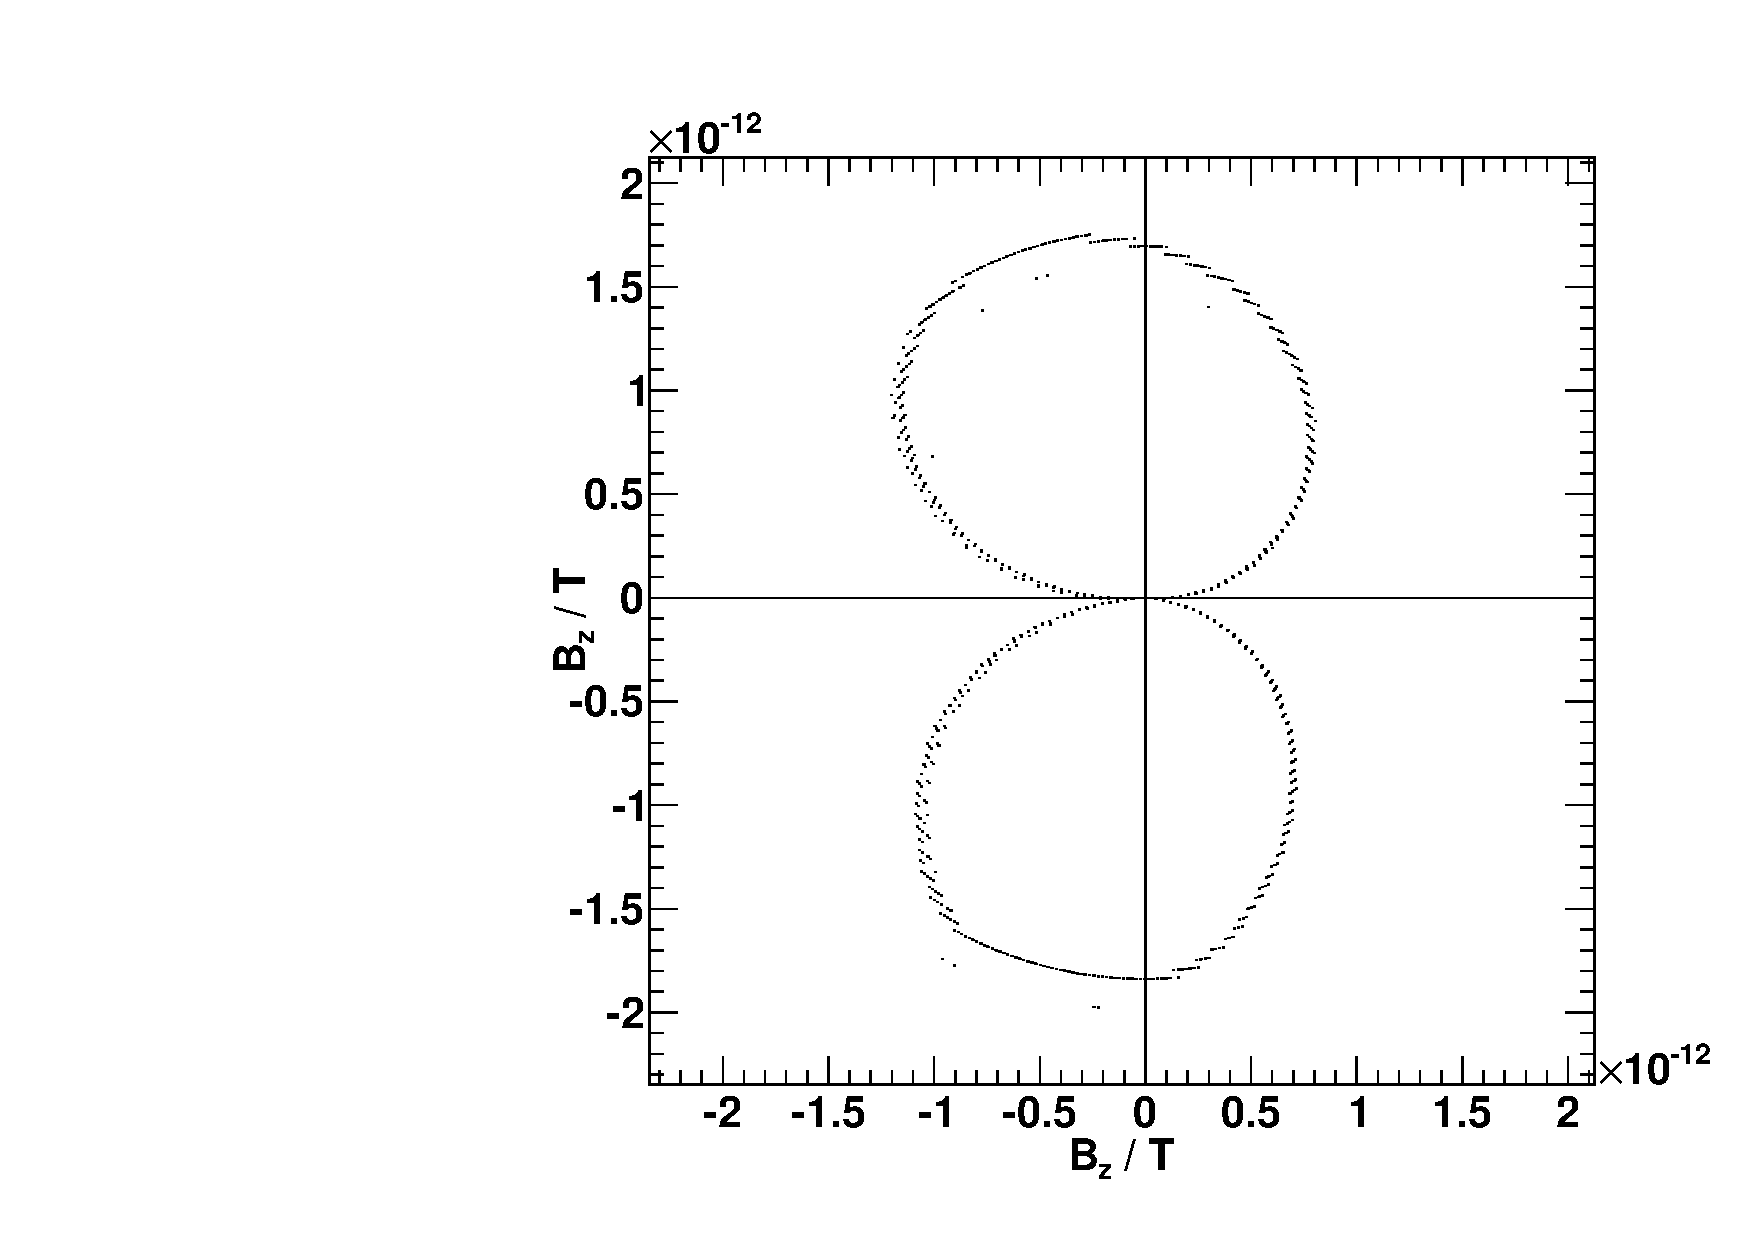
\includegraphics[width=0.35\textwidth]{../img/polar_Magnetspan_45grad.pdf}
  \caption{Bestimmung des Magnetfelds eines Magnetspans und Fit mit Sinusfunktion.}
  \label{img:magnetspan}
\end{center}
\end{figure}
Auch die Messung am Magnetspan wurde gemäß \autoref{eq:fit} gefittet.
Für die Amplitude der Schwingung erhält man
\begin{equation}
A_{\text{St}}=(3.880 \pm 0.005)\, \text{V} \ \, .
\end{equation}
Daraus folgt nach \autoref{eq:AtoB} für die maximale Magnetfeldstärke des Stabmagneten
\begin{equation}
B_{\text{St}} = (47.48 \pm 0.06)\,\text{nT} \ \, .
\end{equation}
Obwohl die Spannungsamplitude hier fast genauso hoch ist wie bei der Messung am Stabmagneten,
ist das berechnete Magnetfeld viel kleiner. Dies liegt an den unterschiedlichen Transferkoeffizienten,
die bei der Messung gewählt wurden.\\ 
Im Gegensatz zum Stabmagneten weicht das Messsignal hier von der Form eines Sinus ab.
Dies ist auch gut in der Polardarstellung zu sehen:
Die Struktur des magnetischen Dipols ist erkennbar, sie ist aber leicht in eine Richtung verformt.
Dies kann damit erklärt werden, dass das Feld des Magnetspans erst im Fernfeld ein Dipolfeld ist.
Nahe an der Probe wird das Feld durch die Oberflächenstruktur des Magnetspans verformt.


\subsubsection{Eisenspan}
\begin{figure}[H]
\begin{center}
  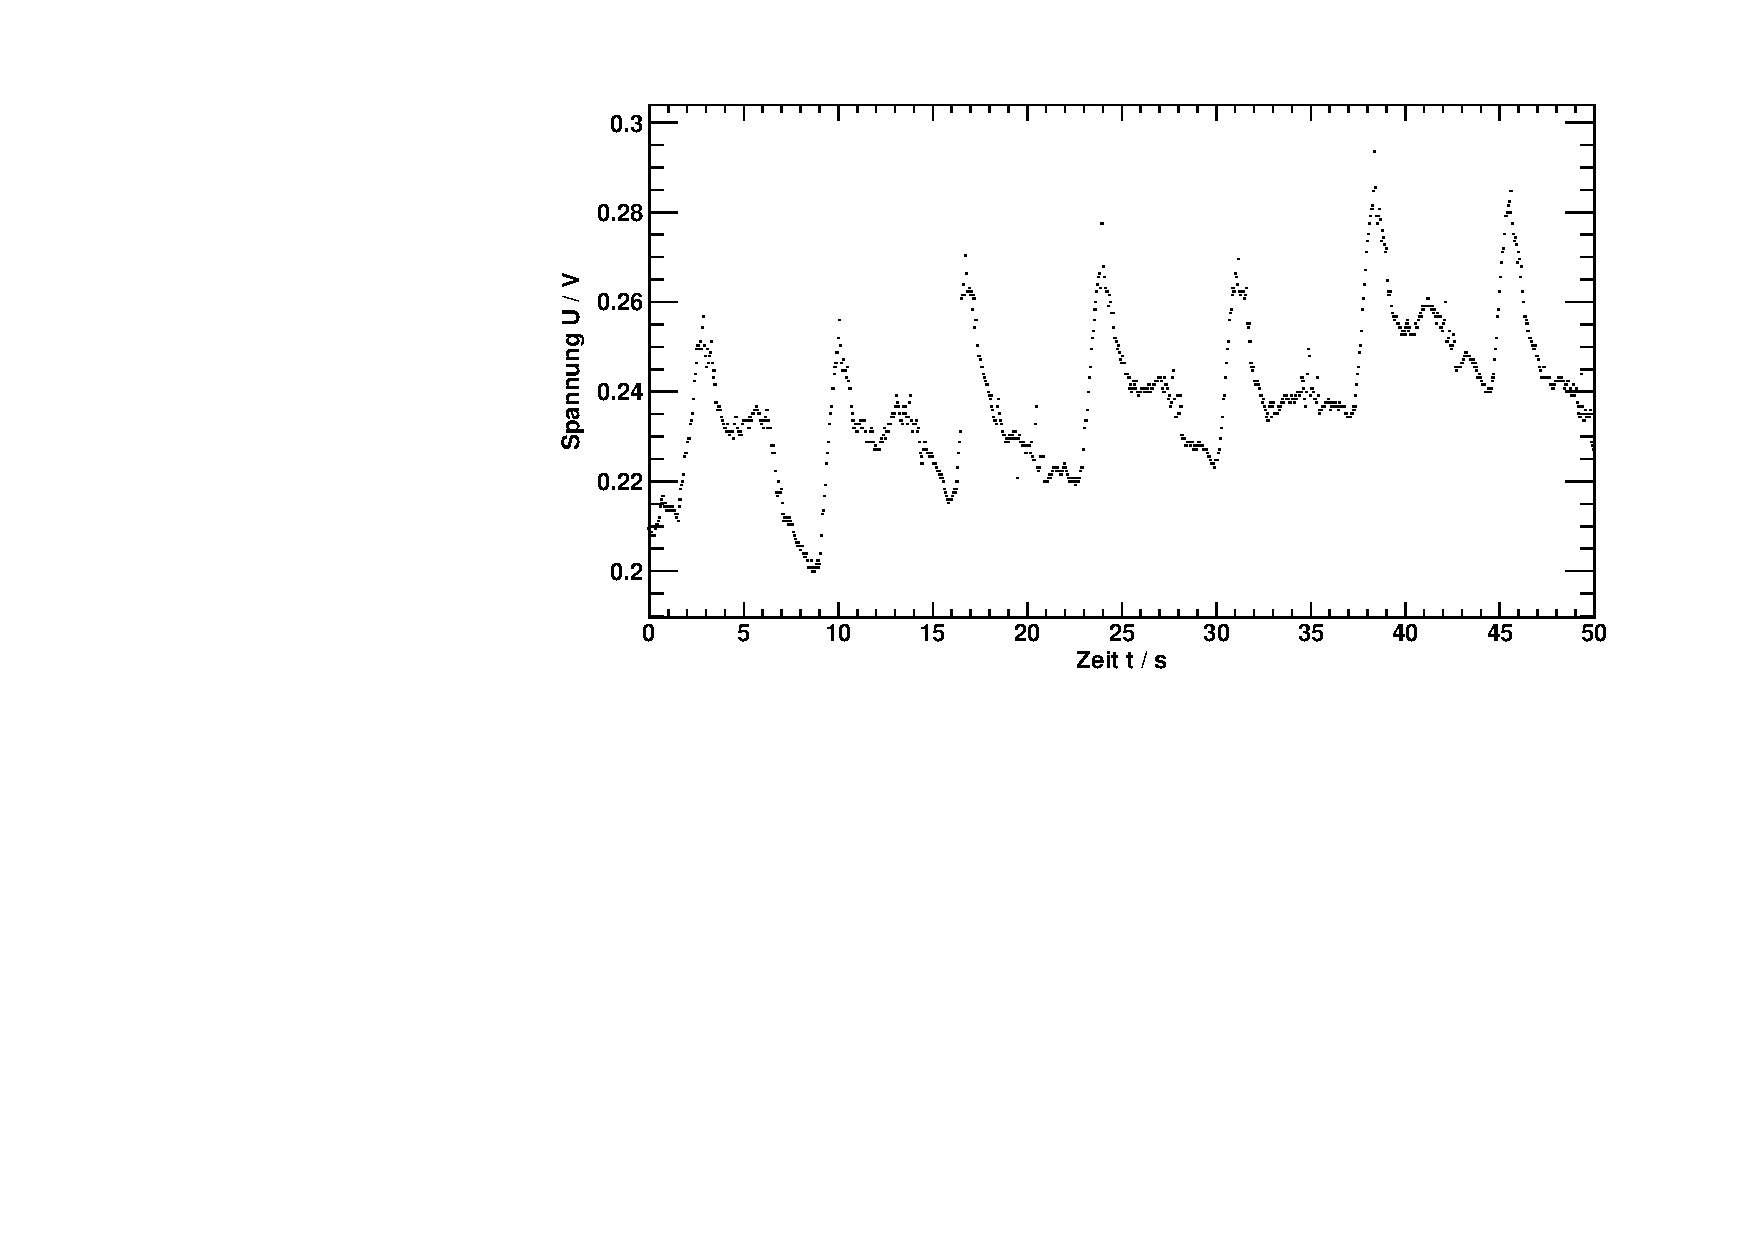
\includegraphics[width=0.64\textwidth]{../img/Fe-Span.pdf}
  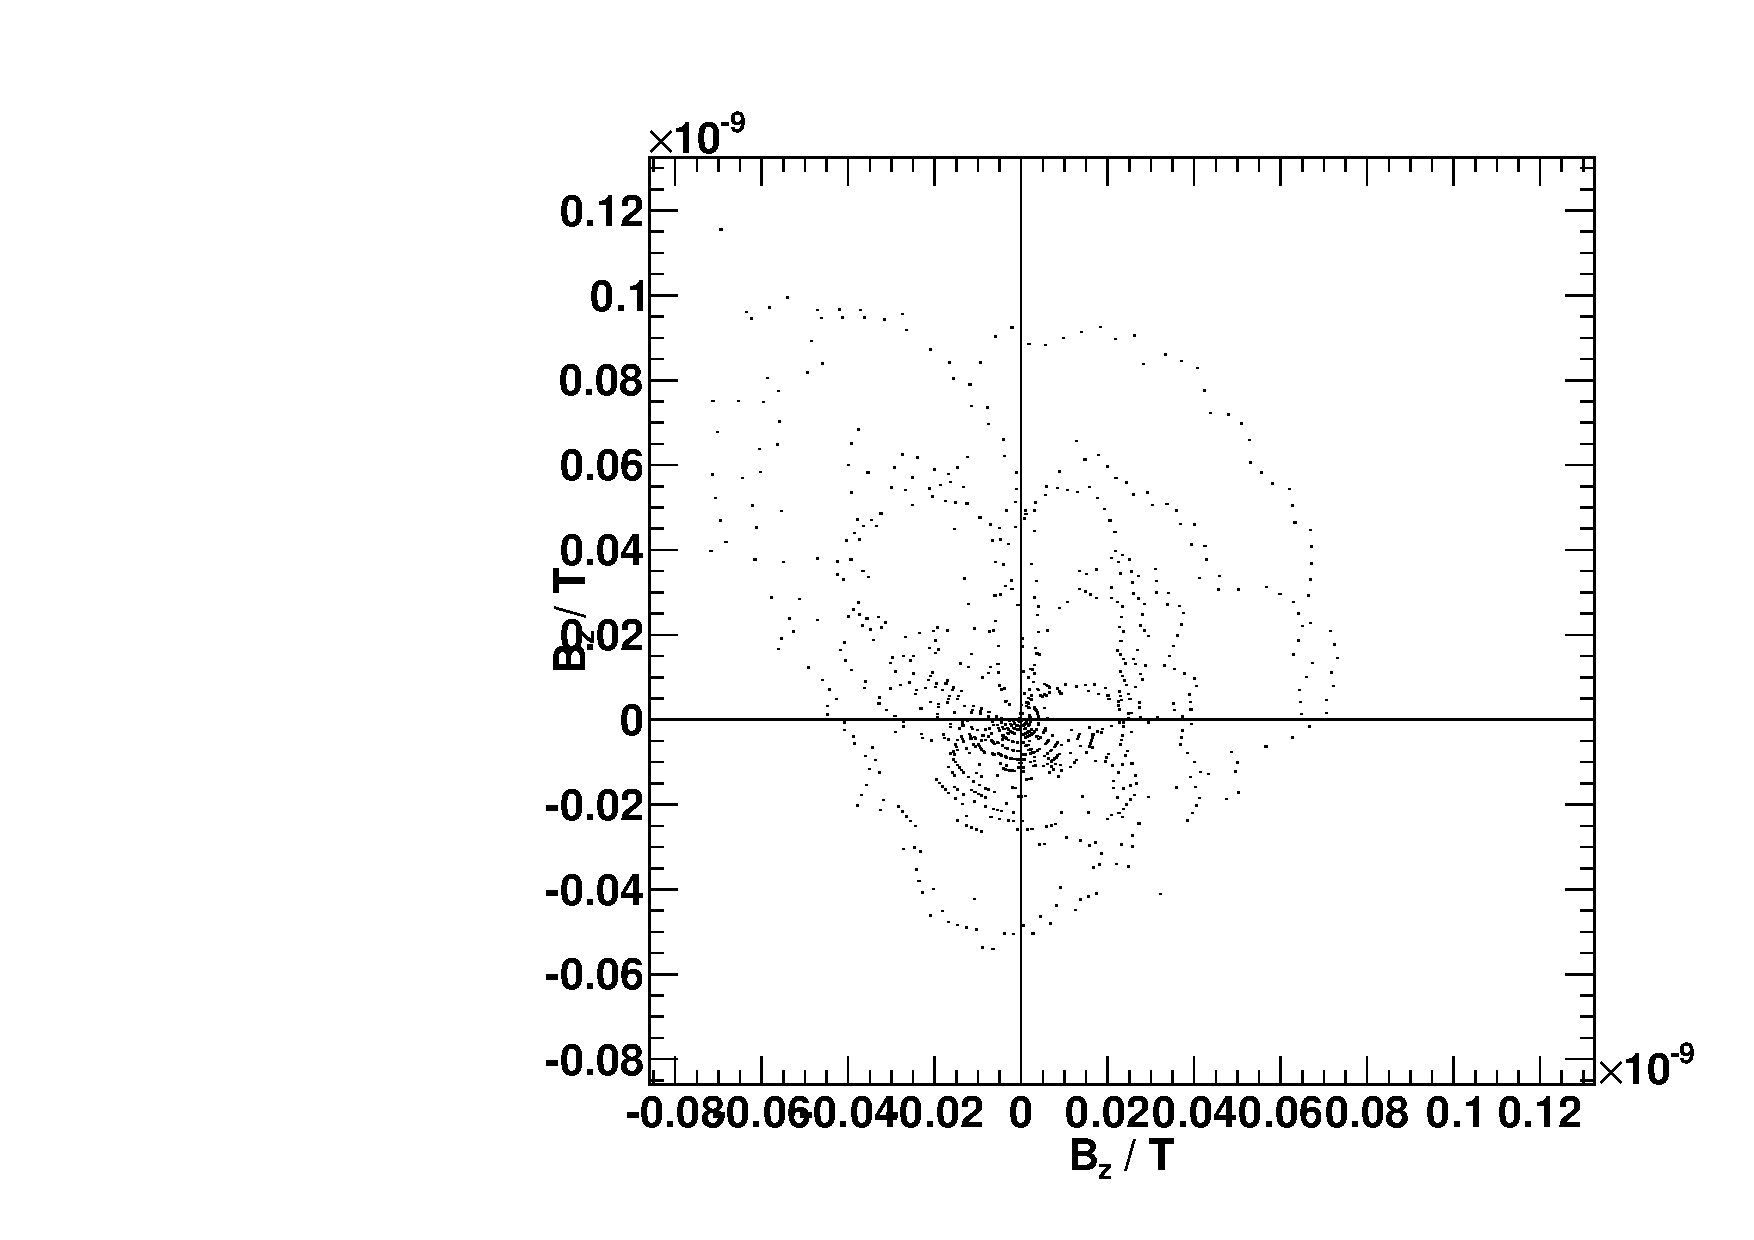
\includegraphics[width=0.35\textwidth]{../img/polar_Fe-Span.pdf}
  \caption{Bestimmung des Magnetfelds eines Eisenspans. Das periodische Signal stammt vermutlich
  vom magnetisierten Probenhalter (\autoref{img:holder}).}
  \label{img:fespan}
\end{center}
\end{figure}
Bei der Messung am Eisenspan ist keine Magnetisierung erkennbar.
Das periodische Signal mit 40\,mV Amplitude wird vermutlich durch den magnetisierten Probenhalter
verursacht (siehe oben).\\
Der Polarplot liefert hier keine eindeutige Aussage.


\subsubsection{Goldplättchen}
\begin{figure}[H]
\begin{center}
  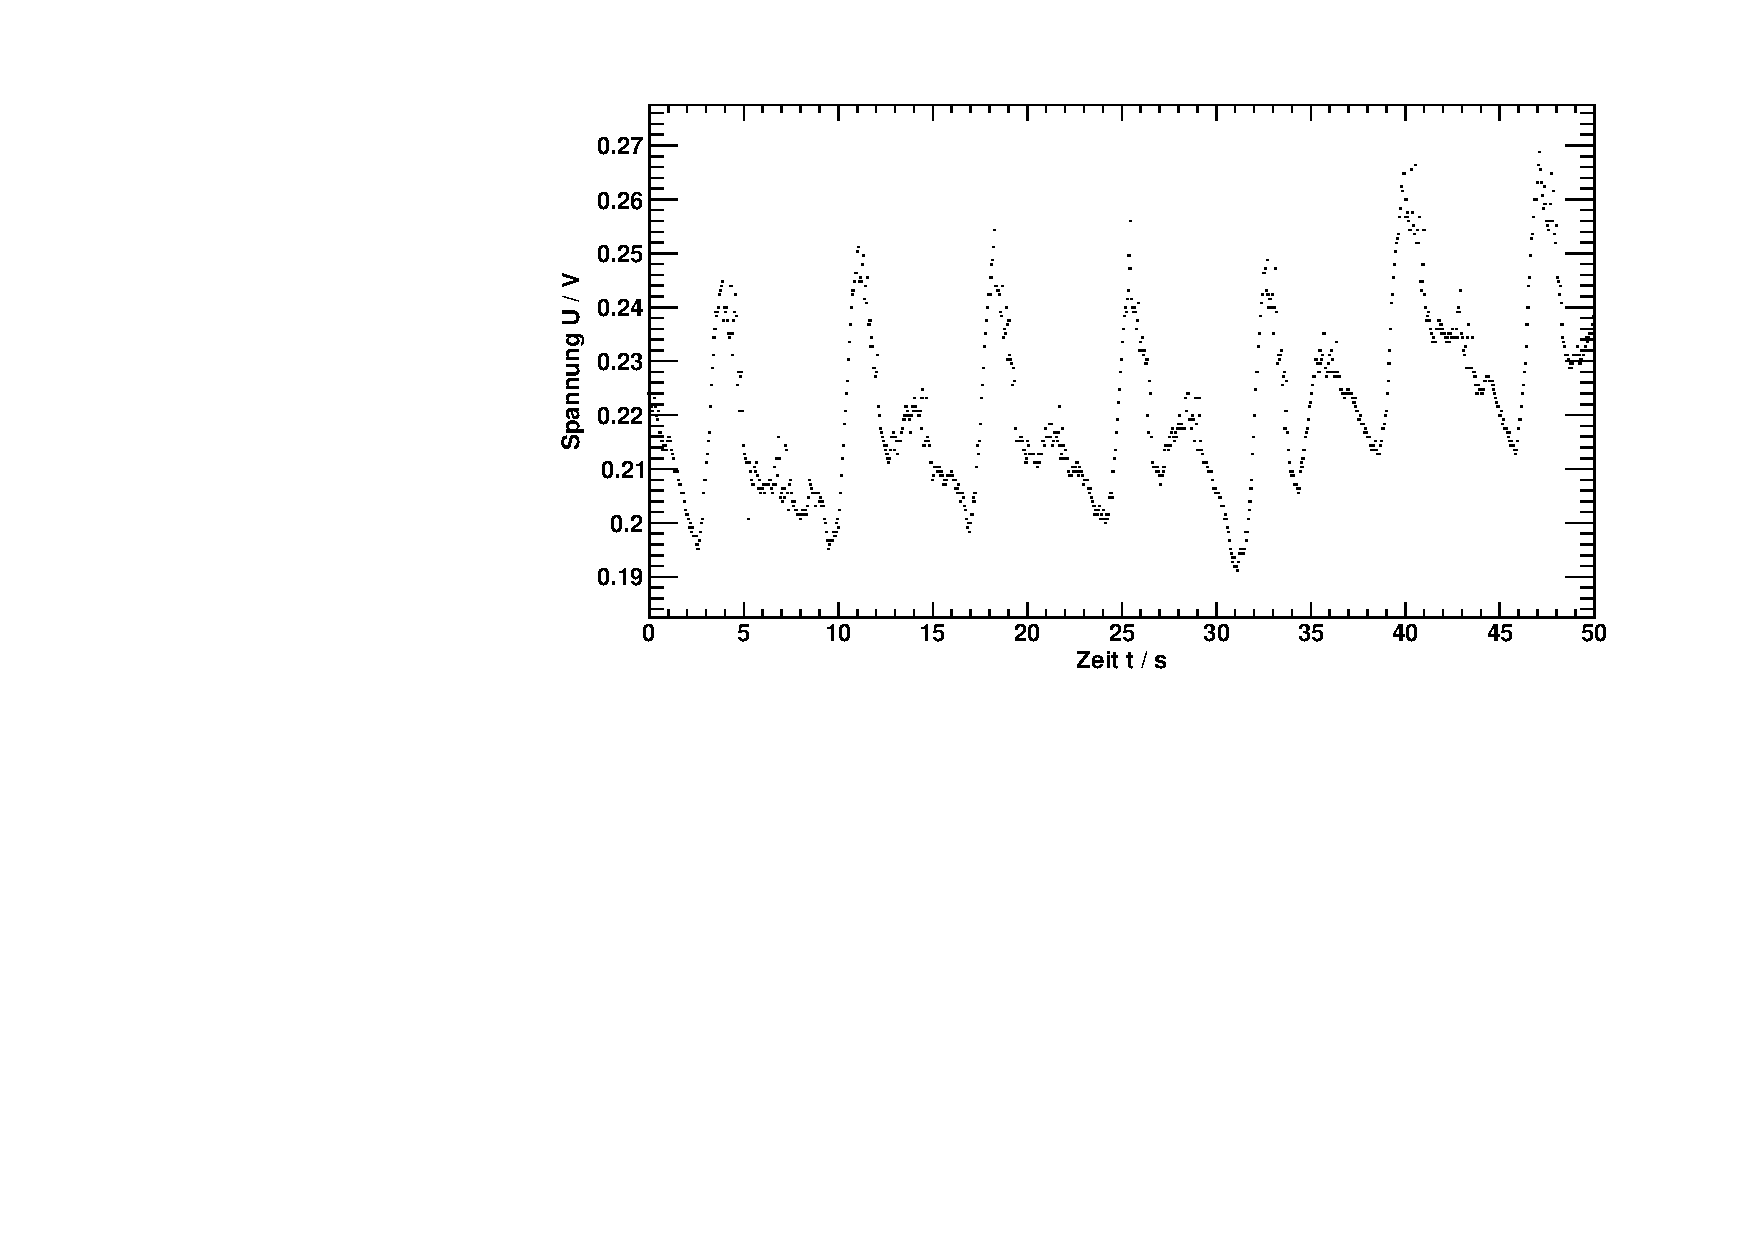
\includegraphics[width=0.64\textwidth]{../img/Au-Plaettchen.pdf}
  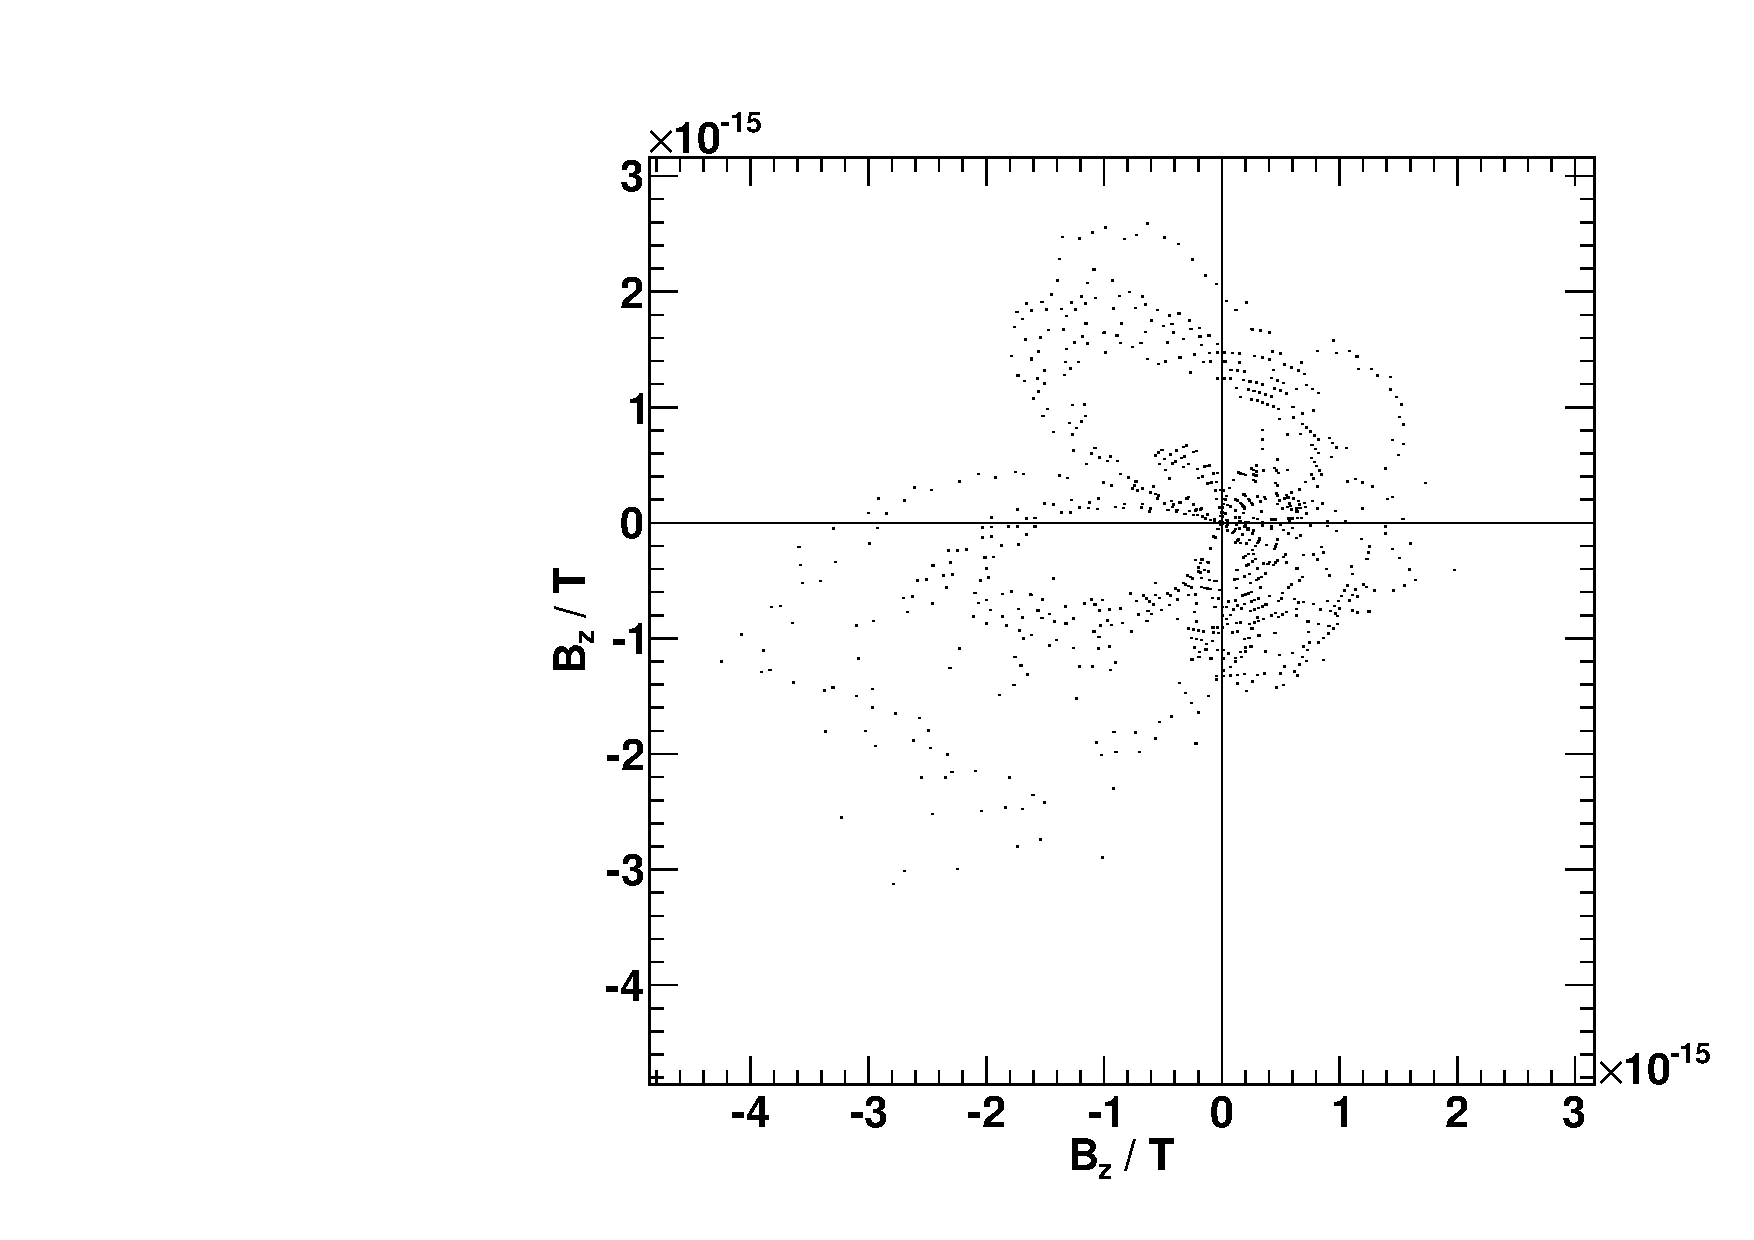
\includegraphics[width=0.35\textwidth]{../img/polar_Au-Plaettchen.pdf}
  \caption{Bestimmung des Magnetfelds eines Goldplättchens. Das periodische Signal stammt vermutlich
  vom magnetisierten Probenhalter (\autoref{img:holder}).}
  \label{img:au}
\end{center}
\end{figure}

Auch das Goldplättchen besitzt kein messbares Magnetfeld,
hier wird ebenfalls nur das Signal des Probenhalters gemessen.

